\documentclass[twoside]{book}

% Packages required by doxygen
\usepackage{fixltx2e}
\usepackage{calc}
\usepackage{doxygen}
\usepackage[export]{adjustbox} % also loads graphicx
\usepackage{graphicx}
\usepackage[utf8]{inputenc}
\usepackage{makeidx}
\usepackage{multicol}
\usepackage{multirow}
\PassOptionsToPackage{warn}{textcomp}
\usepackage{textcomp}
\usepackage[nointegrals]{wasysym}
\usepackage[table]{xcolor}

% Font selection
\usepackage[T1]{fontenc}
\usepackage[scaled=.90]{helvet}
\usepackage{courier}
\usepackage{amssymb}
\usepackage{sectsty}
\renewcommand{\familydefault}{\sfdefault}
\allsectionsfont{%
  \fontseries{bc}\selectfont%
  \color{darkgray}%
}
\renewcommand{\DoxyLabelFont}{%
  \fontseries{bc}\selectfont%
  \color{darkgray}%
}
\newcommand{\+}{\discretionary{\mbox{\scriptsize$\hookleftarrow$}}{}{}}

% Page & text layout
\usepackage{geometry}
\geometry{%
  a4paper,%
  top=2.5cm,%
  bottom=2.5cm,%
  left=2.5cm,%
  right=2.5cm%
}
\tolerance=750
\hfuzz=15pt
\hbadness=750
\setlength{\emergencystretch}{15pt}
\setlength{\parindent}{0cm}
\setlength{\parskip}{3ex plus 2ex minus 2ex}
\makeatletter
\renewcommand{\paragraph}{%
  \@startsection{paragraph}{4}{0ex}{-1.0ex}{1.0ex}{%
    \normalfont\normalsize\bfseries\SS@parafont%
  }%
}
\renewcommand{\subparagraph}{%
  \@startsection{subparagraph}{5}{0ex}{-1.0ex}{1.0ex}{%
    \normalfont\normalsize\bfseries\SS@subparafont%
  }%
}
\makeatother

% Headers & footers
\usepackage{fancyhdr}
\pagestyle{fancyplain}
\fancyhead[LE]{\fancyplain{}{\bfseries\thepage}}
\fancyhead[CE]{\fancyplain{}{}}
\fancyhead[RE]{\fancyplain{}{\bfseries\leftmark}}
\fancyhead[LO]{\fancyplain{}{\bfseries\rightmark}}
\fancyhead[CO]{\fancyplain{}{}}
\fancyhead[RO]{\fancyplain{}{\bfseries\thepage}}
\fancyfoot[LE]{\fancyplain{}{}}
\fancyfoot[CE]{\fancyplain{}{}}
\fancyfoot[RE]{\fancyplain{}{\bfseries\scriptsize Generated by Doxygen }}
\fancyfoot[LO]{\fancyplain{}{\bfseries\scriptsize Generated by Doxygen }}
\fancyfoot[CO]{\fancyplain{}{}}
\fancyfoot[RO]{\fancyplain{}{}}
\renewcommand{\footrulewidth}{0.4pt}
\renewcommand{\chaptermark}[1]{%
  \markboth{#1}{}%
}
\renewcommand{\sectionmark}[1]{%
  \markright{\thesection\ #1}%
}

% Indices & bibliography
\usepackage{natbib}
\usepackage[titles]{tocloft}
\setcounter{tocdepth}{3}
\setcounter{secnumdepth}{5}
\makeindex

% Hyperlinks (required, but should be loaded last)
\usepackage{ifpdf}
\ifpdf
  \usepackage[pdftex,pagebackref=true]{hyperref}
\else
  \usepackage[ps2pdf,pagebackref=true]{hyperref}
\fi
\hypersetup{%
  colorlinks=true,%
  linkcolor=blue,%
  citecolor=blue,%
  unicode%
}

% Custom commands
\newcommand{\clearemptydoublepage}{%
  \newpage{\pagestyle{empty}\cleardoublepage}%
}

\usepackage{caption}
\captionsetup{labelsep=space,justification=centering,font={bf},singlelinecheck=off,skip=4pt,position=top}

%===== C O N T E N T S =====

\begin{document}

% Titlepage & ToC
\hypersetup{pageanchor=false,
             bookmarksnumbered=true,
             pdfencoding=unicode
            }
\pagenumbering{alph}
\begin{titlepage}
\vspace*{7cm}
\begin{center}%
{\Large S\+C\+R\+I\+PT Script (Script$^\wedge$2) \\[1ex]\large 0.\+x }\\
\vspace*{1cm}
{\large Generated by Doxygen 1.8.14}\\
\end{center}
\end{titlepage}
\clearemptydoublepage
\pagenumbering{roman}
\tableofcontents
\clearemptydoublepage
\pagenumbering{arabic}
\hypersetup{pageanchor=true}

%--- Begin generated contents ---
\chapter{Script$^\wedge$2}
\label{md__r_e_a_d_m_e}
\Hypertarget{md__r_e_a_d_m_e}
Serial Chinese Room, Interprocess, and Telemetry (S\+C\+R\+I\+PT) Specification defines A family of technologies, collectively refereed to as Script, that are built on the Chinese Room Abstract Stack Machine (Crabs), S\+C\+R\+I\+PT Software-\/defined Networking Protocol, and S\+C\+R\+I\+PT Script (Script$^\wedge$2 or Script2) and provides\+:


\begin{DoxyItemize}
\item Seam Trees provide low-\/cost in-\/order unit tests for Agile and Issue Driven Development with debug information customized for each tree node.
\item Modern Embedded-\/\+C++11/\+Visual-\/\+C++/\+G\+CC 4.\+7 core with Doxygen A\+PI docs without depreciated libraries.
\item A\+S\+C\+II Data Types and the A\+S\+C\+II Factory operate seamlessly across assembly boundary with optimal R\+AM usage and C\+PU cache performance from R\+O\+M-\/able A\+S\+C\+II Contiguous Objects.
\item Rapid compile time using C Application Binary Interface (A\+BI) with separated C++ templates for cross-\/language bindings.
\item Code automatically formatted to Google C++ Style Guide upon save and formatted to not fight clang-\/format.
\item Deep Internet-\/of-\/\+Things integration using the S\+C\+R\+I\+PT Software Defined Networking Protocol.
\item Modeled after AI philosophy and A\+S\+C\+II mimicry of the Chinese Room Thought Experiment and C0 Control Codes.
\end{DoxyItemize}

\subsection*{A\+S\+C\+II Data Types}

A\+S\+C\+II Data Types provide a suitable replacement for the C++ std library suitable for embedded systems and AI that facilitates\+:


\begin{DoxyItemize}
\item All of the C++ P\+OD types.
\item Year 2038-\/safe 32-\/bit, 64-\/ bit and dual-\/32-\/bit with 16-\/year epoch and sub-\/second tick timestamps.
\item All data types are 64-\/bit aligned so they may be rapidly copied from one system to another on homo-\/endian system.
\item Optional M\+SB variant encoding provides fast data compression similar to U\+T\+F-\/8.
\item Contiguous Objects
\begin{DoxyItemize}
\item U\+T\+F-\/8, U\+T\+F-\/16, and U\+T\+F-\/32 strings.
\item Stack -\/ A stack of P\+OD types in the form of a bounded-\/sized array.
\item Array -\/ A multidimensional array with Stack of dimensions.
\item Loom -\/ A homogeneous array of U\+T\+F-\/8, U\+T\+F-\/16, or U\+T\+F-\/32 strings.
\item Table -\/ A hash table of contiguous mappings.
\item Map -\/ A sparse map of unsigned integers to A\+S\+C\+II Data Types.
\item Book -\/ A multidictionary (i.\+e. unordered map) without hash table.
\item Dictionary -\/ A dictionary of A\+S\+C\+II Data Types with hash table.
\item B-\/\+Sequence -\/ Describes the order and maximum sizes of a Byte-\/\+Sequence of A\+S\+C\+II Data Types.
\item Expression -\/ Asynchronous Chinese Room Script Expressions capable of concurrently executing scripts in multiple language in real-\/time.
\end{DoxyItemize}
\end{DoxyItemize}

\subsection*{Quick Links}


\begin{DoxyItemize}
\item https\+://github.com/kabuki-\/starship/script/blob/master/docs/readme.\+md \char`\"{}\+F\+A\+Q\char`\"{}
\begin{DoxyItemize}
\item {\itshape Frequently asked questions.}
\end{DoxyItemize}
\item https\+://github.com/kabuki-\/starship/script/blob/master/docs/script\+\_\+specification\+\_\+rfc.\+md \char`\"{}\+Script Specification R\+F\+C\char`\"{}
\begin{DoxyItemize}
\item {\itshape Release for Comment for Serial Chinese Room, Interprocess, and Telemetry (S\+C\+R\+I\+PT) Specification.}
\end{DoxyItemize}
\item \href{https://github.com/kabuki-starship/kabuki-toolkit}{\tt Script}
\begin{DoxyItemize}
\item {\itshape Primary repository of the Script, a Script$^\wedge$2 Toolkit.}
\end{DoxyItemize}
\item \href{https://kabuki-starship.github.io/}{\tt Kabuki Starship Website}
\begin{DoxyItemize}
\item $\ast$\+Official Script website. We are currently looking for someone to help us fix the C\+SS on the website. It only works right at $<$ 1024 pixel width so the problem is in the  section.$\ast$
\end{DoxyItemize}
\end{DoxyItemize}

\subsection*{Author}


\begin{DoxyItemize}
\item \href{https://calemccollough.github.io}{\tt Cale Mc\+Collough} $<$\href{mailto:cale.mccollough@gmail.com}{\tt cale.\+mccollough@gmail.\+com}$>$
\end{DoxyItemize}

\subsection*{License}

Copyright 2014-\/18 (C) \href{mailto:calemccollough@gmail.com}{\tt Cale Mc\+Collough} and contributors. All rights reserved (R).

Licensed under the Apache License, Version 2.\+0 (the \char`\"{}\+License\char`\"{}); you may not use this file except in compliance with the License. You may obtain a copy of the License \href{http://www.apache.org/licenses/LICENSE-2.0}{\tt here}.

Unless required by applicable law or agreed to in writing, software distributed under the License is distributed on an \char`\"{}\+A\+S I\+S\char`\"{} B\+A\+S\+IS, W\+I\+T\+H\+O\+UT W\+A\+R\+R\+A\+N\+T\+I\+ES OR C\+O\+N\+D\+I\+T\+I\+O\+NS OF A\+NY K\+I\+ND, either express or implied. See the License for the specific language governing permissions and limitations under the License. 
\chapter{Hierarchical Index}
\section{Class Hierarchy}
This inheritance list is sorted roughly, but not completely, alphabetically\+:\begin{DoxyCompactList}
\item \contentsline{section}{\+\_\+\+:\+:C\+Clock}{\pageref{struct___1_1_c_clock}}{}
\item \contentsline{section}{\+\_\+\+:\+:C\+Object}{\pageref{struct___1_1_c_object}}{}
\item \contentsline{section}{\+\_\+\+:\+:Collection}{\pageref{struct___1_1_collection}}{}
\item \contentsline{section}{\+\_\+\+:\+:C\+Stack$<$ T, UI, SI $>$}{\pageref{struct___1_1_c_stack}}{}
\item \contentsline{section}{\+\_\+\+:\+:Key\+Id}{\pageref{struct___1_1_key_id}}{}
\item \contentsline{section}{\+\_\+\+:\+:Socket}{\pageref{struct___1_1_socket}}{}
\item \contentsline{section}{\+\_\+\+:\+:T\+Binary$<$ Float, UI $>$}{\pageref{class___1_1_t_binary}}{}
\item \contentsline{section}{\+\_\+\+:\+:T\+Center$<$ Char $>$}{\pageref{class___1_1_t_center}}{}
\item \contentsline{section}{\+\_\+\+:\+:T\+Line$<$ Char $>$}{\pageref{struct___1_1_t_line}}{}
\item \contentsline{section}{\+\_\+\+:\+:T\+Line\+String$<$ Char $>$}{\pageref{struct___1_1_t_line_string}}{}
\item \contentsline{section}{\+\_\+\+:\+:T\+Object$<$ Size $>$}{\pageref{class___1_1_t_object}}{}
\item \contentsline{section}{\+\_\+\+:\+:T\+Object$<$ SI $>$}{\pageref{class___1_1_t_object}}{}
\item \contentsline{section}{\+\_\+\+:\+:T\+Right$<$ Char $>$}{\pageref{class___1_1_t_right}}{}
\item \contentsline{section}{\+\_\+\+:\+:T\+Set$<$ T\+Index, T\+Key, T\+Data, T\+Hash $>$}{\pageref{struct___1_1_t_set}}{}
\item \contentsline{section}{\+\_\+\+:\+:T\+Socket$<$ k\+Size\+\_\+, k\+Boundary\+Bit\+Count\+\_\+ $>$}{\pageref{class___1_1_t_socket}}{}
\item \contentsline{section}{\+\_\+\+:\+:Tss}{\pageref{struct___1_1_tss}}{}
\item \contentsline{section}{\+\_\+\+:\+:T\+Stack$<$ T, UI, SI $>$}{\pageref{class___1_1_t_stack}}{}
\item \contentsline{section}{\+\_\+\+:\+:T\+Token$<$ Char $>$}{\pageref{class___1_1_t_token}}{}
\item \contentsline{section}{\+\_\+\+:\+:Tuple2}{\pageref{struct___1_1_tuple2}}{}
\item \contentsline{section}{\+\_\+\+:\+:Tuple3}{\pageref{struct___1_1_tuple3}}{}
\item \contentsline{section}{\+\_\+\+:\+:T\+U\+TF$<$ Char $>$}{\pageref{struct___1_1_t_u_t_f}}{}
\begin{DoxyCompactList}
\item \contentsline{section}{\+\_\+\+:\+:T\+String$<$ Char, Size $>$}{\pageref{class___1_1_t_string}}{}
\end{DoxyCompactList}
\item \contentsline{section}{\+\_\+\+:\+:U\+T\+F1}{\pageref{struct___1_1_u_t_f1}}{}
\item \contentsline{section}{\+\_\+\+:\+:Utf8\+Center}{\pageref{class___1_1_utf8_center}}{}
\item \contentsline{section}{\+\_\+\+:\+:Utf8\+Line}{\pageref{struct___1_1_utf8_line}}{}
\item \contentsline{section}{\+\_\+\+:\+:Utf8\+Line\+String}{\pageref{struct___1_1_utf8_line_string}}{}
\item \contentsline{section}{\+\_\+\+:\+:Utf8\+Right}{\pageref{class___1_1_utf8_right}}{}
\item \contentsline{section}{\+\_\+\+:\+:Utf8\+Text}{\pageref{class___1_1_utf8_text}}{}
\end{DoxyCompactList}

\chapter{Class Index}
\section{Class List}
Here are the classes, structs, unions and interfaces with brief descriptions\+:\begin{DoxyCompactList}
\item\contentsline{section}{\mbox{\hyperlink{struct___1_1_c_clock}{\+\_\+\+::\+C\+Clock}} }{\pageref{struct___1_1_c_clock}}{}
\item\contentsline{section}{\mbox{\hyperlink{struct___1_1_c_object}{\+\_\+\+::\+C\+Object}} }{\pageref{struct___1_1_c_object}}{}
\item\contentsline{section}{\mbox{\hyperlink{struct___1_1_collection}{\+\_\+\+::\+Collection}} }{\pageref{struct___1_1_collection}}{}
\item\contentsline{section}{\mbox{\hyperlink{struct___1_1_c_stack}{\+\_\+\+::\+C\+Stack$<$ T, U\+I, S\+I $>$}} }{\pageref{struct___1_1_c_stack}}{}
\item\contentsline{section}{\mbox{\hyperlink{struct___1_1_key_id}{\+\_\+\+::\+Key\+Id}} }{\pageref{struct___1_1_key_id}}{}
\item\contentsline{section}{\mbox{\hyperlink{struct___1_1_socket}{\+\_\+\+::\+Socket}} }{\pageref{struct___1_1_socket}}{}
\item\contentsline{section}{\mbox{\hyperlink{class___1_1_t_binary}{\+\_\+\+::\+T\+Binary$<$ Float, U\+I $>$}} }{\pageref{class___1_1_t_binary}}{}
\item\contentsline{section}{\mbox{\hyperlink{class___1_1_t_center}{\+\_\+\+::\+T\+Center$<$ Char $>$}} }{\pageref{class___1_1_t_center}}{}
\item\contentsline{section}{\mbox{\hyperlink{struct___1_1_t_line}{\+\_\+\+::\+T\+Line$<$ Char $>$}} }{\pageref{struct___1_1_t_line}}{}
\item\contentsline{section}{\mbox{\hyperlink{struct___1_1_t_line_string}{\+\_\+\+::\+T\+Line\+String$<$ Char $>$}} }{\pageref{struct___1_1_t_line_string}}{}
\item\contentsline{section}{\mbox{\hyperlink{class___1_1_t_object}{\+\_\+\+::\+T\+Object$<$ Size $>$}} }{\pageref{class___1_1_t_object}}{}
\item\contentsline{section}{\mbox{\hyperlink{class___1_1_t_right}{\+\_\+\+::\+T\+Right$<$ Char $>$}} }{\pageref{class___1_1_t_right}}{}
\item\contentsline{section}{\mbox{\hyperlink{struct___1_1_t_set}{\+\_\+\+::\+T\+Set$<$ T\+Index, T\+Key, T\+Data, T\+Hash $>$}} }{\pageref{struct___1_1_t_set}}{}
\item\contentsline{section}{\mbox{\hyperlink{class___1_1_t_socket}{\+\_\+\+::\+T\+Socket$<$ k\+Size\+\_\+, k\+Boundary\+Bit\+Count\+\_\+ $>$}} }{\pageref{class___1_1_t_socket}}{}
\item\contentsline{section}{\mbox{\hyperlink{struct___1_1_tss}{\+\_\+\+::\+Tss}} }{\pageref{struct___1_1_tss}}{}
\item\contentsline{section}{\mbox{\hyperlink{class___1_1_t_stack}{\+\_\+\+::\+T\+Stack$<$ T, U\+I, S\+I $>$}} }{\pageref{class___1_1_t_stack}}{}
\item\contentsline{section}{\mbox{\hyperlink{class___1_1_t_string}{\+\_\+\+::\+T\+String$<$ Char, Size $>$}} }{\pageref{class___1_1_t_string}}{}
\item\contentsline{section}{\mbox{\hyperlink{class___1_1_t_token}{\+\_\+\+::\+T\+Token$<$ Char $>$}} }{\pageref{class___1_1_t_token}}{}
\item\contentsline{section}{\mbox{\hyperlink{struct___1_1_tuple2}{\+\_\+\+::\+Tuple2}} }{\pageref{struct___1_1_tuple2}}{}
\item\contentsline{section}{\mbox{\hyperlink{struct___1_1_tuple3}{\+\_\+\+::\+Tuple3}} }{\pageref{struct___1_1_tuple3}}{}
\item\contentsline{section}{\mbox{\hyperlink{struct___1_1_t_u_t_f}{\+\_\+\+::\+T\+U\+T\+F$<$ Char $>$}} }{\pageref{struct___1_1_t_u_t_f}}{}
\item\contentsline{section}{\mbox{\hyperlink{struct___1_1_u_t_f1}{\+\_\+\+::\+U\+T\+F1}} }{\pageref{struct___1_1_u_t_f1}}{}
\item\contentsline{section}{\mbox{\hyperlink{class___1_1_utf8_center}{\+\_\+\+::\+Utf8\+Center}} }{\pageref{class___1_1_utf8_center}}{}
\item\contentsline{section}{\mbox{\hyperlink{struct___1_1_utf8_line}{\+\_\+\+::\+Utf8\+Line}} }{\pageref{struct___1_1_utf8_line}}{}
\item\contentsline{section}{\mbox{\hyperlink{struct___1_1_utf8_line_string}{\+\_\+\+::\+Utf8\+Line\+String}} }{\pageref{struct___1_1_utf8_line_string}}{}
\item\contentsline{section}{\mbox{\hyperlink{class___1_1_utf8_right}{\+\_\+\+::\+Utf8\+Right}} }{\pageref{class___1_1_utf8_right}}{}
\item\contentsline{section}{\mbox{\hyperlink{class___1_1_utf8_text}{\+\_\+\+::\+Utf8\+Text}} }{\pageref{class___1_1_utf8_text}}{}
\end{DoxyCompactList}

\chapter{File Index}
\section{File List}
Here is a list of all documented files with brief descriptions\+:\begin{DoxyCompactList}
\item\contentsline{section}{{\bfseries 0\+\_\+0\+\_\+0\+\_\+\+\_\+00\+\_\+rng.\+h} }{\pageref{0__0__0____00__rng_8h}}{}
\item\contentsline{section}{{\bfseries 0\+\_\+0\+\_\+0\+\_\+\+\_\+01\+\_\+itos\+\_\+and\+\_\+stoi.\+h} }{\pageref{0__0__0____01__itos__and__stoi_8h}}{}
\item\contentsline{section}{{\bfseries 0\+\_\+0\+\_\+0\+\_\+\+\_\+02\+\_\+ascii\+\_\+strings\+\_\+and\+\_\+socket.\+h} }{\pageref{0__0__0____02__ascii__strings__and__socket_8h}}{}
\item\contentsline{section}{{\bfseries 0\+\_\+0\+\_\+0\+\_\+\+\_\+03\+\_\+ftos\+\_\+and\+\_\+stof.\+h} }{\pageref{0__0__0____03__ftos__and__stof_8h}}{}
\item\contentsline{section}{{\bfseries 0\+\_\+0\+\_\+0\+\_\+\+\_\+04\+\_\+clock.\+h} }{\pageref{0__0__0____04__clock_8h}}{}
\item\contentsline{section}{{\bfseries 0\+\_\+0\+\_\+0\+\_\+\+\_\+05\+\_\+ascii\+\_\+stack.\+h} }{\pageref{0__0__0____05__ascii__stack_8h}}{}
\item\contentsline{section}{{\bfseries 0\+\_\+0\+\_\+0\+\_\+\+\_\+06\+\_\+ascii\+\_\+array.\+h} }{\pageref{0__0__0____06__ascii__array_8h}}{}
\item\contentsline{section}{{\bfseries 0\+\_\+0\+\_\+0\+\_\+\+\_\+07\+\_\+ascii\+\_\+loom.\+h} }{\pageref{0__0__0____07__ascii__loom_8h}}{}
\item\contentsline{section}{{\bfseries 0\+\_\+0\+\_\+0\+\_\+\+\_\+08\+\_\+ascii\+\_\+table.\+h} }{\pageref{0__0__0____08__ascii__table_8h}}{}
\item\contentsline{section}{{\bfseries 0\+\_\+0\+\_\+0\+\_\+\+\_\+09\+\_\+ascii\+\_\+list.\+h} }{\pageref{0__0__0____09__ascii__list_8h}}{}
\item\contentsline{section}{{\bfseries 0\+\_\+0\+\_\+0\+\_\+\+\_\+10\+\_\+ascii\+\_\+map.\+h} }{\pageref{0__0__0____10__ascii__map_8h}}{}
\item\contentsline{section}{{\bfseries 0\+\_\+0\+\_\+0\+\_\+\+\_\+11\+\_\+ascii\+\_\+book.\+h} }{\pageref{0__0__0____11__ascii__book_8h}}{}
\item\contentsline{section}{{\bfseries 0\+\_\+0\+\_\+0\+\_\+\+\_\+12\+\_\+ascii\+\_\+dictionary.\+h} }{\pageref{0__0__0____12__ascii__dictionary_8h}}{}
\item\contentsline{section}{{\bfseries 0\+\_\+0\+\_\+0\+\_\+\+\_\+13\+\_\+room.\+h} }{\pageref{0__0__0____13__room_8h}}{}
\item\contentsline{section}{{\bfseries 0\+\_\+0\+\_\+0\+\_\+script2.\+h} }{\pageref{0__0__0__script2_8h}}{}
\item\contentsline{section}{{\bfseries caddress.\+h} }{\pageref{caddress_8h}}{}
\item\contentsline{section}{{\bfseries cargs.\+h} }{\pageref{cargs_8h}}{}
\item\contentsline{section}{{\bfseries cascii.\+h} }{\pageref{cascii_8h}}{}
\item\contentsline{section}{{\bfseries casciidata.\+h} }{\pageref{casciidata_8h}}{}
\item\contentsline{section}{{\bfseries cbenchmark.\+h} }{\pageref{cbenchmark_8h}}{}
\item\contentsline{section}{{\bfseries cbin.\+h} }{\pageref{cbin_8h}}{}
\item\contentsline{section}{{\bfseries cbinary.\+h} }{\pageref{cbinary_8h}}{}
\item\contentsline{section}{{\bfseries cbout.\+h} }{\pageref{cbout_8h}}{}
\item\contentsline{section}{{\bfseries cbsq.\+h} }{\pageref{cbsq_8h}}{}
\item\contentsline{section}{{\bfseries cbuffer.\+h} }{\pageref{cbuffer_8h}}{}
\item\contentsline{section}{{\bfseries cclock.\+h} }{\pageref{cclock_8h}}{}
\item\contentsline{section}{{\bfseries ccrabs.\+h} }{\pageref{ccrabs_8h}}{}
\item\contentsline{section}{{\bfseries cdoor.\+h} }{\pageref{cdoor_8h}}{}
\item\contentsline{section}{{\bfseries cerror.\+h} }{\pageref{cerror_8h}}{}
\item\contentsline{section}{{\bfseries cevent.\+h} }{\pageref{cevent_8h}}{}
\item\contentsline{section}{{\bfseries cfloor.\+h} }{\pageref{cfloor_8h}}{}
\item\contentsline{section}{{\bfseries chash.\+h} }{\pageref{chash_8h}}{}
\item\contentsline{section}{{\bfseries cinterrupts.\+h} }{\pageref{cinterrupts_8h}}{}
\item\contentsline{section}{{\bfseries citerator.\+h} }{\pageref{citerator_8h}}{}
\item\contentsline{section}{{\bfseries clanguage.\+h} }{\pageref{clanguage_8h}}{}
\item\contentsline{section}{{\bfseries clibrary.\+h} }{\pageref{clibrary_8h}}{}
\item\contentsline{section}{{\bfseries clock.\+h} }{\pageref{clock_8h}}{}
\item\contentsline{section}{{\bfseries cmirror.\+h} }{\pageref{cmirror_8h}}{}
\item\contentsline{section}{{\bfseries cobject.\+h} }{\pageref{cobject_8h}}{}
\item\contentsline{section}{{\bfseries cop.\+h} }{\pageref{cop_8h}}{}
\item\contentsline{section}{{\bfseries coperand.\+h} }{\pageref{coperand_8h}}{}
\item\contentsline{section}{{\bfseries crng.\+h} }{\pageref{crng_8h}}{}
\item\contentsline{section}{{\bfseries croom.\+h} }{\pageref{croom_8h}}{}
\item\contentsline{section}{{\bfseries csio.\+h} }{\pageref{csio_8h}}{}
\item\contentsline{section}{{\bfseries cslot.\+h} }{\pageref{cslot_8h}}{}
\item\contentsline{section}{{\bfseries csocket.\+h} }{\pageref{csocket_8h}}{}
\item\contentsline{section}{{\bfseries cstack.\+h} }{\pageref{cstack_8h}}{}
\item\contentsline{section}{{\bfseries ctest.\+h} }{\pageref{ctest_8h}}{}
\item\contentsline{section}{{\bfseries cutf.\+h} }{\pageref{cutf_8h}}{}
\item\contentsline{section}{{\bfseries cutf1.\+h} }{\pageref{cutf1_8h}}{}
\item\contentsline{section}{{\bfseries cutf2.\+h} }{\pageref{cutf2_8h}}{}
\item\contentsline{section}{{\bfseries cutf4.\+h} }{\pageref{cutf4_8h}}{}
\item\contentsline{section}{{\bfseries cvarint.\+h} }{\pageref{cvarint_8h}}{}
\item\contentsline{section}{{\bfseries cvk.\+h} }{\pageref{cvk_8h}}{}
\item\contentsline{section}{{\bfseries cwall.\+h} }{\pageref{cwall_8h}}{}
\item\contentsline{section}{{\bfseries global.\+h} }{\pageref{global_8h}}{}
\item\contentsline{section}{{\bfseries global\+\_\+config.\+h} }{\pageref{global__config_8h}}{}
\item\contentsline{section}{{\bfseries header.\+h} }{\pageref{header_8h}}{}
\item\contentsline{section}{{\bfseries pch.\+h} }{\pageref{pch_8h}}{}
\item\contentsline{section}{{\bfseries public.\+h} }{\pageref{public_8h}}{}
\item\contentsline{section}{\mbox{\hyperlink{script2__morsecode_8cc}{script2\+\_\+morsecode.\+cc}} }{\pageref{script2__morsecode_8cc}}{}
\item\contentsline{section}{{\bfseries tarray.\+h} }{\pageref{tarray_8h}}{}
\item\contentsline{section}{{\bfseries tasciidata.\+h} }{\pageref{tasciidata_8h}}{}
\item\contentsline{section}{{\bfseries tbenchmark.\+h} }{\pageref{tbenchmark_8h}}{}
\item\contentsline{section}{{\bfseries tbinary.\+h} }{\pageref{tbinary_8h}}{}
\item\contentsline{section}{{\bfseries tbook.\+h} }{\pageref{tbook_8h}}{}
\item\contentsline{section}{{\bfseries tclock.\+h} }{\pageref{tclock_8h}}{}
\item\contentsline{section}{{\bfseries tdictionary.\+h} }{\pageref{tdictionary_8h}}{}
\item\contentsline{section}{{\bfseries thash.\+h} }{\pageref{thash_8h}}{}
\item\contentsline{section}{{\bfseries tlist.\+h} }{\pageref{tlist_8h}}{}
\item\contentsline{section}{{\bfseries tloom.\+h} }{\pageref{tloom_8h}}{}
\item\contentsline{section}{{\bfseries tmap.\+h} }{\pageref{tmap_8h}}{}
\item\contentsline{section}{{\bfseries tobject.\+h} }{\pageref{tobject_8h}}{}
\item\contentsline{section}{{\bfseries tset.\+h} }{\pageref{tset_8h}}{}
\item\contentsline{section}{{\bfseries tsocket.\+h} }{\pageref{tsocket_8h}}{}
\item\contentsline{section}{{\bfseries tstack.\+h} }{\pageref{tstack_8h}}{}
\item\contentsline{section}{{\bfseries ttable.\+h} }{\pageref{ttable_8h}}{}
\item\contentsline{section}{{\bfseries ttest.\+h} }{\pageref{ttest_8h}}{}
\item\contentsline{section}{{\bfseries tutf.\+h} }{\pageref{tutf_8h}}{}
\end{DoxyCompactList}

\chapter{Class Documentation}
\hypertarget{struct___1_1_c_clock}{}\section{\+\_\+\+:\+:C\+Clock Struct Reference}
\label{struct___1_1_c_clock}\index{\+\_\+\+::\+C\+Clock@{\+\_\+\+::\+C\+Clock}}
\subsection*{Public Member Functions}
\begin{DoxyCompactItemize}
\item 
\mbox{\Hypertarget{struct___1_1_c_clock_a82cca31e51f6cf9fab5deb4ebb47f817}\label{struct___1_1_c_clock_a82cca31e51f6cf9fab5deb4ebb47f817}} 
{\bfseries C\+Clock} (T\+MS time)
\item 
\mbox{\Hypertarget{struct___1_1_c_clock_a5844dc98d153e1679b1c0a5f1fae94f8}\label{struct___1_1_c_clock_a5844dc98d153e1679b1c0a5f1fae94f8}} 
{\bfseries C\+Clock} (T\+ME time)
\item 
\mbox{\Hypertarget{struct___1_1_c_clock_a006c8ffd330283924926bcfc3208e1b5}\label{struct___1_1_c_clock_a006c8ffd330283924926bcfc3208e1b5}} 
void {\bfseries Set\+Time} (T\+MS t)
\item 
\mbox{\Hypertarget{struct___1_1_c_clock_a6cb1ec6d1faf7939b8a6ac21684b708c}\label{struct___1_1_c_clock_a6cb1ec6d1faf7939b8a6ac21684b708c}} 
void {\bfseries Set\+Time} (T\+ME t)
\end{DoxyCompactItemize}
\subsection*{Public Attributes}
\begin{DoxyCompactItemize}
\item 
\mbox{\Hypertarget{struct___1_1_c_clock_ae46829f86685aa5d7d84fb0e8d7b3c77}\label{struct___1_1_c_clock_ae46829f86685aa5d7d84fb0e8d7b3c77}} 
int {\bfseries second}
\item 
\mbox{\Hypertarget{struct___1_1_c_clock_ab96039908c7bd47abf5e3970755c343d}\label{struct___1_1_c_clock_ab96039908c7bd47abf5e3970755c343d}} 
int {\bfseries minute}
\item 
\mbox{\Hypertarget{struct___1_1_c_clock_a05b9992b1883ea5d70b121bc036c748e}\label{struct___1_1_c_clock_a05b9992b1883ea5d70b121bc036c748e}} 
int {\bfseries hour}
\item 
\mbox{\Hypertarget{struct___1_1_c_clock_a11f2cc83dd258f949ae0397f78dc66ef}\label{struct___1_1_c_clock_a11f2cc83dd258f949ae0397f78dc66ef}} 
int {\bfseries day}
\item 
\mbox{\Hypertarget{struct___1_1_c_clock_a35bb6160b6e523a82c249f63e88cb395}\label{struct___1_1_c_clock_a35bb6160b6e523a82c249f63e88cb395}} 
int {\bfseries month}
\item 
\mbox{\Hypertarget{struct___1_1_c_clock_a6c76e464b46a73ee6b177eed1bbf9335}\label{struct___1_1_c_clock_a6c76e464b46a73ee6b177eed1bbf9335}} 
int {\bfseries year}
\end{DoxyCompactItemize}


The documentation for this struct was generated from the following files\+:\begin{DoxyCompactItemize}
\item 
cclock.\+h\item 
script2\+\_\+clock.\+cc\end{DoxyCompactItemize}

\hypertarget{struct___1_1_c_object}{}\section{\+\_\+\+:\+:C\+Object Struct Reference}
\label{struct___1_1_c_object}\index{\+\_\+\+::\+C\+Object@{\+\_\+\+::\+C\+Object}}
\subsection*{Public Attributes}
\begin{DoxyCompactItemize}
\item 
\mbox{\Hypertarget{struct___1_1_c_object_a247735495ff4a9594627296db63e95d6}\label{struct___1_1_c_object_a247735495ff4a9594627296db63e95d6}} 
U\+IW $\ast$ {\bfseries begin}
\item 
\mbox{\Hypertarget{struct___1_1_c_object_aa29f5ba995fd7a2d5626391d7718041c}\label{struct___1_1_c_object_aa29f5ba995fd7a2d5626391d7718041c}} 
Ascii\+Factory {\bfseries factory}
\end{DoxyCompactItemize}


The documentation for this struct was generated from the following file\+:\begin{DoxyCompactItemize}
\item 
cobject.\+h\end{DoxyCompactItemize}

\hypertarget{struct___1_1_collection}{}\section{\+\_\+\+:\+:Collection Struct Reference}
\label{struct___1_1_collection}\index{\+\_\+\+::\+Collection@{\+\_\+\+::\+Collection}}
\subsection*{Public Member Functions}
\begin{DoxyCompactItemize}
\item 
\mbox{\Hypertarget{struct___1_1_collection_a2e2a2a7a7ed399e787b55cb5a16278fd}\label{struct___1_1_collection_a2e2a2a7a7ed399e787b55cb5a16278fd}} 
virtual void {\bfseries Clear} ()=0
\item 
\mbox{\Hypertarget{struct___1_1_collection_a3575fe9c157fede5038dbef555e4dcf2}\label{struct___1_1_collection_a3575fe9c157fede5038dbef555e4dcf2}} 
virtual void {\bfseries Wipe} ()=0
\item 
\mbox{\Hypertarget{struct___1_1_collection_a434f86ce2b04d22701fa642fe1c751c0}\label{struct___1_1_collection_a434f86ce2b04d22701fa642fe1c751c0}} 
virtual B\+OL {\bfseries Push} (Ascii\+Type type, void $\ast$value)=0
\item 
\mbox{\Hypertarget{struct___1_1_collection_ab19089046a0a71466a670ffde06a1c90}\label{struct___1_1_collection_ab19089046a0a71466a670ffde06a1c90}} 
virtual B\+OL {\bfseries Push} (Ascii\+Type type, void $\ast$value, const char $\ast$key)=0
\item 
\mbox{\Hypertarget{struct___1_1_collection_a2952c1b0f706475dc934f1ab77b68140}\label{struct___1_1_collection_a2952c1b0f706475dc934f1ab77b68140}} 
virtual B\+OL {\bfseries Merge} (\mbox{\hyperlink{struct___1_1_collection}{Collection}} $\ast$collection)=0
\item 
\mbox{\Hypertarget{struct___1_1_collection_ae3ff784577f8a2b216d8184e754b4130}\label{struct___1_1_collection_ae3ff784577f8a2b216d8184e754b4130}} 
virtual B\+OL {\bfseries Remove} (\mbox{\hyperlink{struct___1_1_tuple2}{Tuple2}} $\ast$tuple)=0
\item 
\mbox{\Hypertarget{struct___1_1_collection_af838f8aaed0c997fd641c8d0573d8f07}\label{struct___1_1_collection_af838f8aaed0c997fd641c8d0573d8f07}} 
virtual B\+OL {\bfseries Remove} (U\+IW)=0
\item 
\mbox{\Hypertarget{struct___1_1_collection_a4a40d810a39178ce85ddb9a417a17925}\label{struct___1_1_collection_a4a40d810a39178ce85ddb9a417a17925}} 
virtual B\+OL {\bfseries Remove} (const char $\ast$key)=0
\item 
\mbox{\Hypertarget{struct___1_1_collection_aed4556e61d25cf78ed8b8ffff5544a25}\label{struct___1_1_collection_aed4556e61d25cf78ed8b8ffff5544a25}} 
virtual void $\ast$ {\bfseries Get} (U\+IW index)=0
\item 
\mbox{\Hypertarget{struct___1_1_collection_a312bda685ccc810998d7f74c52a0780b}\label{struct___1_1_collection_a312bda685ccc810998d7f74c52a0780b}} 
virtual void $\ast$ {\bfseries Get} (const char $\ast$key)=0
\item 
\mbox{\Hypertarget{struct___1_1_collection_a9fc9a0581e1194f380e88f6fd5dffe58}\label{struct___1_1_collection_a9fc9a0581e1194f380e88f6fd5dffe58}} 
virtual U\+IW {\bfseries Find\+Index} (const char $\ast$key)=0
\item 
\mbox{\Hypertarget{struct___1_1_collection_afd0337f030477dcd2096406c1726d016}\label{struct___1_1_collection_afd0337f030477dcd2096406c1726d016}} 
virtual U\+IW {\bfseries Find\+Index} (Ascii\+Type type, void $\ast$value)=0
\item 
\mbox{\Hypertarget{struct___1_1_collection_a4f65730da45fdfa070e0104430496390}\label{struct___1_1_collection_a4f65730da45fdfa070e0104430496390}} 
virtual U\+IW {\bfseries Get\+Size} ()=0
\item 
\mbox{\Hypertarget{struct___1_1_collection_a698ca48dbc2870f1f2bed1344441b826}\label{struct___1_1_collection_a698ca48dbc2870f1f2bed1344441b826}} 
virtual U\+IW {\bfseries Get\+Size\+Width} ()=0
\item 
\mbox{\Hypertarget{struct___1_1_collection_a422d6d496174cc9fd2f6d03956ef5a03}\label{struct___1_1_collection_a422d6d496174cc9fd2f6d03956ef5a03}} 
virtual \mbox{\hyperlink{struct___1_1_u_t_f1}{U\+T\+F1}} \& {\bfseries Print} (\mbox{\hyperlink{struct___1_1_u_t_f1}{U\+T\+F1}} \&out\+\_\+)=0
\end{DoxyCompactItemize}


The documentation for this struct was generated from the following file\+:\begin{DoxyCompactItemize}
\item 
tset.\+h\end{DoxyCompactItemize}

\hypertarget{struct___1_1_c_stack}{}\section{\+\_\+\+:\+:C\+Stack$<$ T, UI, SI $>$ Struct Template Reference}
\label{struct___1_1_c_stack}\index{\+\_\+\+::\+C\+Stack$<$ T, U\+I, S\+I $>$@{\+\_\+\+::\+C\+Stack$<$ T, U\+I, S\+I $>$}}
\subsection*{Public Attributes}
\begin{DoxyCompactItemize}
\item 
\mbox{\Hypertarget{struct___1_1_c_stack_a2cb844909ae77cdd3ebf258e5596a449}\label{struct___1_1_c_stack_a2cb844909ae77cdd3ebf258e5596a449}} 
UI {\bfseries size\+\_\+array}
\item 
\mbox{\Hypertarget{struct___1_1_c_stack_ad804024f8b065d7a0da602ae1489ff94}\label{struct___1_1_c_stack_ad804024f8b065d7a0da602ae1489ff94}} 
UI {\bfseries size\+\_\+stack}
\item 
\mbox{\Hypertarget{struct___1_1_c_stack_a8c39cd7bd00e3e82734983906120a0a6}\label{struct___1_1_c_stack_a8c39cd7bd00e3e82734983906120a0a6}} 
SI {\bfseries count\+\_\+max}
\item 
\mbox{\Hypertarget{struct___1_1_c_stack_ad709d196c244f5abad0b0ce2da7b9d3f}\label{struct___1_1_c_stack_ad709d196c244f5abad0b0ce2da7b9d3f}} 
SI {\bfseries count}
\end{DoxyCompactItemize}


The documentation for this struct was generated from the following files\+:\begin{DoxyCompactItemize}
\item 
cstack.\+h\item 
tstack.\+h\end{DoxyCompactItemize}

\hypertarget{struct___1_1_key_id}{}\section{\+\_\+\+:\+:Key\+Id Struct Reference}
\label{struct___1_1_key_id}\index{\+\_\+\+::\+Key\+Id@{\+\_\+\+::\+Key\+Id}}
\subsection*{Public Member Functions}
\begin{DoxyCompactItemize}
\item 
\mbox{\Hypertarget{struct___1_1_key_id_afab53d92b982b95325d887b0577d26d3}\label{struct___1_1_key_id_afab53d92b982b95325d887b0577d26d3}} 
{\bfseries Key\+Id} (V\+K\+Code code, const char $\ast$label)
\item 
\mbox{\Hypertarget{struct___1_1_key_id_a405e65a86aca56b2170d73755e16f428}\label{struct___1_1_key_id_a405e65a86aca56b2170d73755e16f428}} 
void {\bfseries Reprogram\+Console} ()
\end{DoxyCompactItemize}
\subsection*{Public Attributes}
\begin{DoxyCompactItemize}
\item 
\mbox{\Hypertarget{struct___1_1_key_id_a36f4e0ed8ccd1e7e1fc57dd09c94efaa}\label{struct___1_1_key_id_a36f4e0ed8ccd1e7e1fc57dd09c94efaa}} 
int {\bfseries vk\+\_\+code}
\item 
\mbox{\Hypertarget{struct___1_1_key_id_a721cdedf1c6461604e013c8a473d657b}\label{struct___1_1_key_id_a721cdedf1c6461604e013c8a473d657b}} 
const char $\ast$ {\bfseries label}
\item 
\mbox{\Hypertarget{struct___1_1_key_id_a270e818e63622cd91f5da9fac26c1ce4}\label{struct___1_1_key_id_a270e818e63622cd91f5da9fac26c1ce4}} 
const char $\ast$ {\bfseries description}
\end{DoxyCompactItemize}


The documentation for this struct was generated from the following files\+:\begin{DoxyCompactItemize}
\item 
cvk.\+h\item 
script2\+\_\+vk.\+cc\end{DoxyCompactItemize}

\hypertarget{struct___1_1_socket}{}\section{\+\_\+\+:\+:Socket Struct Reference}
\label{struct___1_1_socket}\index{\+\_\+\+::\+Socket@{\+\_\+\+::\+Socket}}
\subsection*{Public Member Functions}
\begin{DoxyCompactItemize}
\item 
\mbox{\Hypertarget{struct___1_1_socket_a923b7fab144b6904243e6d810e0bd8bb}\label{struct___1_1_socket_a923b7fab144b6904243e6d810e0bd8bb}} 
{\bfseries Socket} (void $\ast$begin, void $\ast$end)
\item 
\mbox{\Hypertarget{struct___1_1_socket_a6097aeb259bfc581f43b751f86831550}\label{struct___1_1_socket_a6097aeb259bfc581f43b751f86831550}} 
{\bfseries Socket} (void $\ast$begin, S\+IW size)
\item 
\mbox{\Hypertarget{struct___1_1_socket_a6b2080b00a83d7046dbde89725035100}\label{struct___1_1_socket_a6b2080b00a83d7046dbde89725035100}} 
{\bfseries Socket} (const \mbox{\hyperlink{struct___1_1_socket}{Socket}} \&other)
\item 
\mbox{\Hypertarget{struct___1_1_socket_a03847729267b665839b62697d048fe92}\label{struct___1_1_socket_a03847729267b665839b62697d048fe92}} 
\mbox{\hyperlink{struct___1_1_socket}{Socket}} \& {\bfseries operator=} (const \mbox{\hyperlink{struct___1_1_socket}{Socket}} \&other)
\end{DoxyCompactItemize}
\subsection*{Public Attributes}
\begin{DoxyCompactItemize}
\item 
\mbox{\Hypertarget{struct___1_1_socket_a56b74fec8beff4f276c3ce242756ecb9}\label{struct___1_1_socket_a56b74fec8beff4f276c3ce242756ecb9}} 
char $\ast$ {\bfseries begin}
\item 
\mbox{\Hypertarget{struct___1_1_socket_ab2a4f34d0657744f04de538fed2b7369}\label{struct___1_1_socket_ab2a4f34d0657744f04de538fed2b7369}} 
char $\ast$ {\bfseries end}
\end{DoxyCompactItemize}


The documentation for this struct was generated from the following files\+:\begin{DoxyCompactItemize}
\item 
csocket.\+h\item 
script2\+\_\+socket.\+cc\end{DoxyCompactItemize}

\hypertarget{class___1_1_t_binary}{}\section{\+\_\+\+:\+:T\+Binary$<$ Float, UI $>$ Class Template Reference}
\label{class___1_1_t_binary}\index{\+\_\+\+::\+T\+Binary$<$ Float, U\+I $>$@{\+\_\+\+::\+T\+Binary$<$ Float, U\+I $>$}}
\subsection*{Public Types}
\begin{DoxyCompactItemize}
\item 
\mbox{\Hypertarget{class___1_1_t_binary_af5a08d4a78e453bf384ff85e4aac2118}\label{class___1_1_t_binary_af5a08d4a78e453bf384ff85e4aac2118}} 
enum \{ \newline
{\bfseries k\+Size} = sizeof(Float), 
{\bfseries k\+Size\+Bits} = k\+Size $\ast$ 8, 
{\bfseries k\+M\+Sb\+Index} = k\+Size\+Bits -\/ 1, 
{\bfseries k\+String\+Length\+Max} = 24, 
\newline
{\bfseries k\+Exponent\+Size\+Bits}, 
{\bfseries k\+Coefficient\+Size} = k\+Size\+Bits -\/ k\+Exponent\+Size\+Bits -\/ 1, 
{\bfseries k\+Mantissa\+Size} = k\+Size\+Bits -\/ k\+Exponent\+Size\+Bits -\/ 2, 
{\bfseries k\+Exponent\+Mask\+Unshifted} = ($\sim$((UI)0)) $>$$>$ (k\+Size\+Bits -\/ k\+Exponent\+Size\+Bits), 
\newline
{\bfseries k\+Exponent\+Bias} = k\+Exponent\+Mask\+Unshifted + k\+Coefficient\+Size, 
{\bfseries k\+Exponent\+Min} = -\/k\+Exponent\+Bias
 \}
\end{DoxyCompactItemize}
\subsection*{Public Member Functions}
\begin{DoxyCompactItemize}
\item 
\mbox{\Hypertarget{class___1_1_t_binary_a55a35e15c413d2f9db4e6c454e39c8c4}\label{class___1_1_t_binary_a55a35e15c413d2f9db4e6c454e39c8c4}} 
{\bfseries T\+Binary} (Float binary)
\item 
\mbox{\Hypertarget{class___1_1_t_binary_a2344024a8ad45fc1894de16bebcda229}\label{class___1_1_t_binary_a2344024a8ad45fc1894de16bebcda229}} 
{\bfseries T\+Binary} (UI f, S\+I4 e)
\item 
\mbox{\Hypertarget{class___1_1_t_binary_a8198a43d80a948ba714c9730aef78983}\label{class___1_1_t_binary_a8198a43d80a948ba714c9730aef78983}} 
{\bfseries T\+Binary} (const \mbox{\hyperlink{class___1_1_t_binary}{T\+Binary}} a, const \mbox{\hyperlink{class___1_1_t_binary}{T\+Binary}} b)
\end{DoxyCompactItemize}
\subsection*{Static Public Member Functions}
\begin{DoxyCompactItemize}
\item 
\mbox{\Hypertarget{class___1_1_t_binary_a5381e4c8503392d8b67f1d508015885d}\label{class___1_1_t_binary_a5381e4c8503392d8b67f1d508015885d}} 
static int {\bfseries Foo} ()
\item 
\mbox{\Hypertarget{class___1_1_t_binary_a01666dd15a7d07d967d284539e454c36}\label{class___1_1_t_binary_a01666dd15a7d07d967d284539e454c36}} 
static UI {\bfseries Coefficient} (UI decimal)
\item 
\mbox{\Hypertarget{class___1_1_t_binary_a0bfe64689496f819502cb921aa73facf}\label{class___1_1_t_binary_a0bfe64689496f819502cb921aa73facf}} 
static UI {\bfseries Exponent} (UI decimal)
\item 
\mbox{\Hypertarget{class___1_1_t_binary_afaa6d73364479f2a85260196f37da5e0}\label{class___1_1_t_binary_afaa6d73364479f2a85260196f37da5e0}} 
{\footnotesize template$<$typename Char  = char$>$ }\\static Char $\ast$ {\bfseries Print} (Char $\ast$buffer, Char $\ast$end, Float value)
\item 
\mbox{\Hypertarget{class___1_1_t_binary_a600b913209ca4b431719fa5c236edf12}\label{class___1_1_t_binary_a600b913209ca4b431719fa5c236edf12}} 
{\footnotesize template$<$typename UI  = U\+IW$>$ }\\static UI {\bfseries Na\+N\+Unsigned} ()
\item 
\mbox{\Hypertarget{class___1_1_t_binary_ac639e4f36586dfab6817a0129f319e12}\label{class___1_1_t_binary_ac639e4f36586dfab6817a0129f319e12}} 
{\footnotesize template$<$typename SI , typename UI $>$ }\\static SI {\bfseries T\+Na\+N\+Signed} ()
\item 
\mbox{\Hypertarget{class___1_1_t_binary_a6560a784914abf79600196c975df0d95}\label{class___1_1_t_binary_a6560a784914abf79600196c975df0d95}} 
static \mbox{\hyperlink{class___1_1_t_binary}{T\+Binary}} {\bfseries I\+E\+E\+E754\+Pow10} (S\+I4 e, S\+I4 \&k)
\end{DoxyCompactItemize}


The documentation for this class was generated from the following file\+:\begin{DoxyCompactItemize}
\item 
tbinary.\+h\end{DoxyCompactItemize}

\hypertarget{class___1_1_t_center}{}\section{\+\_\+\+:\+:T\+Center$<$ Char $>$ Class Template Reference}
\label{class___1_1_t_center}\index{\+\_\+\+::\+T\+Center$<$ Char $>$@{\+\_\+\+::\+T\+Center$<$ Char $>$}}
\subsection*{Public Member Functions}
\begin{DoxyCompactItemize}
\item 
\mbox{\Hypertarget{class___1_1_t_center_a834ea8bf14a24797ed89c242f92d9b70}\label{class___1_1_t_center_a834ea8bf14a24797ed89c242f92d9b70}} 
{\bfseries T\+Center} (const Char $\ast$string, int column\+\_\+count)
\item 
\mbox{\Hypertarget{class___1_1_t_center_aa999e05e0a65e6adb98b32b473601274}\label{class___1_1_t_center_aa999e05e0a65e6adb98b32b473601274}} 
{\bfseries T\+Center} (S\+I4 value, int column\+\_\+count)
\item 
\mbox{\Hypertarget{class___1_1_t_center_aee9440c4d00cae71b9e35d057a3e8d90}\label{class___1_1_t_center_aee9440c4d00cae71b9e35d057a3e8d90}} 
{\bfseries T\+Center} (U\+I4 value, int column\+\_\+count)
\item 
\mbox{\Hypertarget{class___1_1_t_center_a5e86b0c5fad0898181ec4f9ab5368a2b}\label{class___1_1_t_center_a5e86b0c5fad0898181ec4f9ab5368a2b}} 
{\bfseries T\+Center} (S\+I8 value, int column\+\_\+count)
\item 
\mbox{\Hypertarget{class___1_1_t_center_a3de299cbfc6105db6225b6c53d44c5ef}\label{class___1_1_t_center_a3de299cbfc6105db6225b6c53d44c5ef}} 
{\bfseries T\+Center} (U\+I8 value, int column\+\_\+count)
\item 
\mbox{\Hypertarget{class___1_1_t_center_a8bd3de195af875121eb74472e16753ed}\label{class___1_1_t_center_a8bd3de195af875121eb74472e16753ed}} 
{\bfseries T\+Center} (F\+LT value, int column\+\_\+count)
\item 
\mbox{\Hypertarget{class___1_1_t_center_a88cdfed91f788c665ef08a7950b85c63}\label{class___1_1_t_center_a88cdfed91f788c665ef08a7950b85c63}} 
{\bfseries T\+Center} (D\+BL value, int column\+\_\+count)
\item 
\mbox{\Hypertarget{class___1_1_t_center_a8c0d0187c54ac8391e67e2c74fbacc6c}\label{class___1_1_t_center_a8c0d0187c54ac8391e67e2c74fbacc6c}} 
const Char $\ast$ {\bfseries String} ()
\item 
\mbox{\Hypertarget{class___1_1_t_center_a319e3301ab3c6f1221e20ec9a6220c03}\label{class___1_1_t_center_a319e3301ab3c6f1221e20ec9a6220c03}} 
int {\bfseries Get\+Column\+Count} ()
\end{DoxyCompactItemize}


The documentation for this class was generated from the following file\+:\begin{DoxyCompactItemize}
\item 
tutf.\+h\end{DoxyCompactItemize}

\hypertarget{struct___1_1_t_line}{}\section{\+\_\+\+:\+:T\+Line$<$ Char $>$ Struct Template Reference}
\label{struct___1_1_t_line}\index{\+\_\+\+::\+T\+Line$<$ Char $>$@{\+\_\+\+::\+T\+Line$<$ Char $>$}}
\subsection*{Public Member Functions}
\begin{DoxyCompactItemize}
\item 
\mbox{\Hypertarget{struct___1_1_t_line_acf706a08fa8c78f0be00f2768d36bad8}\label{struct___1_1_t_line_acf706a08fa8c78f0be00f2768d36bad8}} 
{\bfseries T\+Line} (Char token, int column\+\_\+count)
\end{DoxyCompactItemize}
\subsection*{Public Attributes}
\begin{DoxyCompactItemize}
\item 
\mbox{\Hypertarget{struct___1_1_t_line_ac437d948bf14b8d7f0dd0e9f6328ae01}\label{struct___1_1_t_line_ac437d948bf14b8d7f0dd0e9f6328ae01}} 
Char {\bfseries token}
\item 
\mbox{\Hypertarget{struct___1_1_t_line_a054c711434445108137e9e84c8a3e794}\label{struct___1_1_t_line_a054c711434445108137e9e84c8a3e794}} 
int {\bfseries column\+\_\+count}
\end{DoxyCompactItemize}


The documentation for this struct was generated from the following file\+:\begin{DoxyCompactItemize}
\item 
tutf.\+h\end{DoxyCompactItemize}

\hypertarget{struct___1_1_t_line_string}{}\section{\+\_\+\+:\+:T\+Line\+String$<$ Char $>$ Struct Template Reference}
\label{struct___1_1_t_line_string}\index{\+\_\+\+::\+T\+Line\+String$<$ Char $>$@{\+\_\+\+::\+T\+Line\+String$<$ Char $>$}}
\subsection*{Public Member Functions}
\begin{DoxyCompactItemize}
\item 
\mbox{\Hypertarget{struct___1_1_t_line_string_ab3f2579c372c01dad25d4690d2c09729}\label{struct___1_1_t_line_string_ab3f2579c372c01dad25d4690d2c09729}} 
{\bfseries T\+Line\+String} (const Char $\ast$string, int column\+\_\+count)
\end{DoxyCompactItemize}
\subsection*{Public Attributes}
\begin{DoxyCompactItemize}
\item 
\mbox{\Hypertarget{struct___1_1_t_line_string_af986867250068f36eca87444c77dd4f0}\label{struct___1_1_t_line_string_af986867250068f36eca87444c77dd4f0}} 
const Char $\ast$ {\bfseries string}
\item 
\mbox{\Hypertarget{struct___1_1_t_line_string_af5d1d906573cf24639e3ffbc4a1a7063}\label{struct___1_1_t_line_string_af5d1d906573cf24639e3ffbc4a1a7063}} 
int {\bfseries column\+\_\+count}
\end{DoxyCompactItemize}


The documentation for this struct was generated from the following file\+:\begin{DoxyCompactItemize}
\item 
tutf.\+h\end{DoxyCompactItemize}

\hypertarget{class___1_1_t_object}{}\section{\+\_\+\+:\+:T\+Object$<$ Size $>$ Class Template Reference}
\label{class___1_1_t_object}\index{\+\_\+\+::\+T\+Object$<$ Size $>$@{\+\_\+\+::\+T\+Object$<$ Size $>$}}
\subsection*{Public Member Functions}
\begin{DoxyCompactItemize}
\item 
\mbox{\Hypertarget{class___1_1_t_object_ab66313143c93737dc65406a1c26d18b6}\label{class___1_1_t_object_ab66313143c93737dc65406a1c26d18b6}} 
{\bfseries T\+Object} (Ascii\+Factory destructor)
\item 
\mbox{\Hypertarget{class___1_1_t_object_a03fb0b9ab63401aab298ec35146481f6}\label{class___1_1_t_object_a03fb0b9ab63401aab298ec35146481f6}} 
{\bfseries T\+Object} (Size size, Ascii\+Factory destructor=nullptr)
\item 
\mbox{\Hypertarget{class___1_1_t_object_a1cabcbc1b77526710d914e6dbab6038e}\label{class___1_1_t_object_a1cabcbc1b77526710d914e6dbab6038e}} 
{\bfseries T\+Object} (Size size, U\+IW $\ast$buffer, Ascii\+Factory destructor=nullptr)
\item 
\mbox{\Hypertarget{class___1_1_t_object_a8715af5669f93f72bcf927c02c05698e}\label{class___1_1_t_object_a8715af5669f93f72bcf927c02c05698e}} 
U\+IW $\ast$ {\bfseries Begin} ()
\item 
\mbox{\Hypertarget{class___1_1_t_object_af8b5a63d74793675ac77438573d5370c}\label{class___1_1_t_object_af8b5a63d74793675ac77438573d5370c}} 
U\+IW $\ast$ {\bfseries Set\+Begin} (U\+IW $\ast$buffer)
\item 
\mbox{\Hypertarget{class___1_1_t_object_a6823952bcd0510820b87cb48cc8f032c}\label{class___1_1_t_object_a6823952bcd0510820b87cb48cc8f032c}} 
U\+IW $\ast$ {\bfseries Get\+Start} ()
\item 
\mbox{\Hypertarget{class___1_1_t_object_aa07ab6d1984edf2551ccde4ee4646ec0}\label{class___1_1_t_object_aa07ab6d1984edf2551ccde4ee4646ec0}} 
char $\ast$ {\bfseries Get\+Stop} ()
\item 
\mbox{\Hypertarget{class___1_1_t_object_a965cbdc8be82d0e642b8a016d6befcb7}\label{class___1_1_t_object_a965cbdc8be82d0e642b8a016d6befcb7}} 
Size {\bfseries Get\+Size} ()
\item 
\mbox{\Hypertarget{class___1_1_t_object_a9179aa66e7f300bf2706d4099d2cb8dc}\label{class___1_1_t_object_a9179aa66e7f300bf2706d4099d2cb8dc}} 
Ascii\+Factory {\bfseries Get\+Factory} ()
\item 
\mbox{\Hypertarget{class___1_1_t_object_a46ef3097bab2a912c3c311c2e1227066}\label{class___1_1_t_object_a46ef3097bab2a912c3c311c2e1227066}} 
\mbox{\hyperlink{struct___1_1_c_object}{C\+Object}} \& {\bfseries O\+BJ} ()
\end{DoxyCompactItemize}


The documentation for this class was generated from the following file\+:\begin{DoxyCompactItemize}
\item 
tobject.\+h\end{DoxyCompactItemize}

\hypertarget{class___1_1_t_right}{}\section{\+\_\+\+:\+:T\+Right$<$ Char $>$ Class Template Reference}
\label{class___1_1_t_right}\index{\+\_\+\+::\+T\+Right$<$ Char $>$@{\+\_\+\+::\+T\+Right$<$ Char $>$}}
\subsection*{Public Member Functions}
\begin{DoxyCompactItemize}
\item 
\mbox{\Hypertarget{class___1_1_t_right_a05b7b633ef1e7930d94ea45b85e1f846}\label{class___1_1_t_right_a05b7b633ef1e7930d94ea45b85e1f846}} 
{\bfseries T\+Right} (const Char $\ast$string, int column\+\_\+count)
\item 
\mbox{\Hypertarget{class___1_1_t_right_afe816ae4779b9d9029caf02f51fc9072}\label{class___1_1_t_right_afe816ae4779b9d9029caf02f51fc9072}} 
{\bfseries T\+Right} (S\+I4 value, int column\+\_\+count)
\item 
\mbox{\Hypertarget{class___1_1_t_right_a7a65c4473fef0f1e430af4e59469be9a}\label{class___1_1_t_right_a7a65c4473fef0f1e430af4e59469be9a}} 
{\bfseries T\+Right} (U\+I4 value, int column\+\_\+count)
\item 
\mbox{\Hypertarget{class___1_1_t_right_a76249e397a5e6beaef6f2fb94f0b1880}\label{class___1_1_t_right_a76249e397a5e6beaef6f2fb94f0b1880}} 
{\bfseries T\+Right} (S\+I8 value, int column\+\_\+count)
\item 
\mbox{\Hypertarget{class___1_1_t_right_a125675b236ecb73098e8ca1a86074548}\label{class___1_1_t_right_a125675b236ecb73098e8ca1a86074548}} 
{\bfseries T\+Right} (U\+I8 value, int column\+\_\+count)
\item 
\mbox{\Hypertarget{class___1_1_t_right_a5ec20d43ef43f0409c07f5ae8f326677}\label{class___1_1_t_right_a5ec20d43ef43f0409c07f5ae8f326677}} 
{\bfseries T\+Right} (F\+LT value, int column\+\_\+count)
\item 
\mbox{\Hypertarget{class___1_1_t_right_af88222306339a29324e5c83cef14e41d}\label{class___1_1_t_right_af88222306339a29324e5c83cef14e41d}} 
{\bfseries T\+Right} (D\+BL value, int column\+\_\+count)
\item 
\mbox{\Hypertarget{class___1_1_t_right_ab2033b3a057b857513914407e0657b4a}\label{class___1_1_t_right_ab2033b3a057b857513914407e0657b4a}} 
const Char $\ast$ {\bfseries String} ()
\item 
\mbox{\Hypertarget{class___1_1_t_right_a6b5d836ab8db39b3493dfd2eeadfd898}\label{class___1_1_t_right_a6b5d836ab8db39b3493dfd2eeadfd898}} 
int {\bfseries Get\+Column\+Count} ()
\end{DoxyCompactItemize}


The documentation for this class was generated from the following file\+:\begin{DoxyCompactItemize}
\item 
tutf.\+h\end{DoxyCompactItemize}

\hypertarget{struct___1_1_t_set}{}\section{\+\_\+\+:\+:T\+Set$<$ T\+Index, T\+Key, T\+Data, T\+Hash $>$ Struct Template Reference}
\label{struct___1_1_t_set}\index{\+\_\+\+::\+T\+Set$<$ T\+Index, T\+Key, T\+Data, T\+Hash $>$@{\+\_\+\+::\+T\+Set$<$ T\+Index, T\+Key, T\+Data, T\+Hash $>$}}
\subsection*{Public Attributes}
\begin{DoxyCompactItemize}
\item 
\mbox{\Hypertarget{struct___1_1_t_set_a7e0c5e6d9871a09c692bec2c40103c11}\label{struct___1_1_t_set_a7e0c5e6d9871a09c692bec2c40103c11}} 
T\+Data {\bfseries size}
\item 
\mbox{\Hypertarget{struct___1_1_t_set_a245872eea0c8cdd3783b240153c19641}\label{struct___1_1_t_set_a245872eea0c8cdd3783b240153c19641}} 
T\+Key {\bfseries table\+\_\+size}
\item 
\mbox{\Hypertarget{struct___1_1_t_set_a63dac2a240775013d9f65c3acdaefce3}\label{struct___1_1_t_set_a63dac2a240775013d9f65c3acdaefce3}} 
T\+Key {\bfseries size\+\_\+pile}
\item 
\mbox{\Hypertarget{struct___1_1_t_set_a8735fd1260cb438c0bf7e97fb1e7923f}\label{struct___1_1_t_set_a8735fd1260cb438c0bf7e97fb1e7923f}} 
T\+Index {\bfseries item\+\_\+count}
\item 
\mbox{\Hypertarget{struct___1_1_t_set_a463abcab414ff6b33ef3bfde27d8894b}\label{struct___1_1_t_set_a463abcab414ff6b33ef3bfde27d8894b}} 
T\+Index {\bfseries count\+\_\+max}
\end{DoxyCompactItemize}


The documentation for this struct was generated from the following file\+:\begin{DoxyCompactItemize}
\item 
tset.\+h\end{DoxyCompactItemize}

\hypertarget{class___1_1_t_socket}{}\section{\+\_\+\+:\+:T\+Socket$<$ k\+Size\+\_\+, k\+Boundary\+Bit\+Count\+\_\+ $>$ Class Template Reference}
\label{class___1_1_t_socket}\index{\+\_\+\+::\+T\+Socket$<$ k\+Size\+\_\+, k\+Boundary\+Bit\+Count\+\_\+ $>$@{\+\_\+\+::\+T\+Socket$<$ k\+Size\+\_\+, k\+Boundary\+Bit\+Count\+\_\+ $>$}}
\subsection*{Public Types}
\begin{DoxyCompactItemize}
\item 
\mbox{\Hypertarget{class___1_1_t_socket_afff9c7fae8a8b0806846b352db264d02}\label{class___1_1_t_socket_afff9c7fae8a8b0806846b352db264d02}} 
enum \{ {\bfseries k\+Size} = k\+Size\+\_\+, 
{\bfseries k\+Size\+Unaligned} = k\+Size + k\+Boundary\+Bit\+Count\+\_\+, 
{\bfseries k\+Boundary\+Bit\+Count} = k\+Boundary\+Bit\+Count\+\_\+
 \}
\end{DoxyCompactItemize}
\subsection*{Public Member Functions}
\begin{DoxyCompactItemize}
\item 
\mbox{\Hypertarget{class___1_1_t_socket_a1ab41cb60896e42b7449f630a3cef13a}\label{class___1_1_t_socket_a1ab41cb60896e42b7449f630a3cef13a}} 
char $\ast$ {\bfseries Begin} ()
\item 
\mbox{\Hypertarget{class___1_1_t_socket_a90699751c579439af0b64d98186339c7}\label{class___1_1_t_socket_a90699751c579439af0b64d98186339c7}} 
char $\ast$ {\bfseries End} ()
\item 
\mbox{\Hypertarget{class___1_1_t_socket_aa08a16617d9ae4a0c4c8b15d26e1f0c6}\label{class___1_1_t_socket_aa08a16617d9ae4a0c4c8b15d26e1f0c6}} 
{\footnotesize template$<$typename T $>$ }\\T $\ast$ {\bfseries Start} ()
\end{DoxyCompactItemize}


The documentation for this class was generated from the following file\+:\begin{DoxyCompactItemize}
\item 
tsocket.\+h\end{DoxyCompactItemize}

\hypertarget{struct___1_1_tss}{}\section{\+\_\+\+:\+:Tss Struct Reference}
\label{struct___1_1_tss}\index{\+\_\+\+::\+Tss@{\+\_\+\+::\+Tss}}
\subsection*{Public Attributes}
\begin{DoxyCompactItemize}
\item 
\mbox{\Hypertarget{struct___1_1_tss_a35a63a33e02cd25e0d9e1b77b9d5f698}\label{struct___1_1_tss_a35a63a33e02cd25e0d9e1b77b9d5f698}} 
T\+MS {\bfseries seconds}
\item 
\mbox{\Hypertarget{struct___1_1_tss_a7a6f22ad49f9b9b1ed80ea9928c8abb8}\label{struct___1_1_tss_a7a6f22ad49f9b9b1ed80ea9928c8abb8}} 
U\+I4 {\bfseries ticks}
\end{DoxyCompactItemize}


The documentation for this struct was generated from the following file\+:\begin{DoxyCompactItemize}
\item 
cclock.\+h\end{DoxyCompactItemize}

\hypertarget{class___1_1_t_stack}{}\section{\+\_\+\+:\+:T\+Stack$<$ T, UI, SI $>$ Class Template Reference}
\label{class___1_1_t_stack}\index{\+\_\+\+::\+T\+Stack$<$ T, U\+I, S\+I $>$@{\+\_\+\+::\+T\+Stack$<$ T, U\+I, S\+I $>$}}
\subsection*{Public Member Functions}
\begin{DoxyCompactItemize}
\item 
\mbox{\Hypertarget{class___1_1_t_stack_a790c10c5af73eb3d910b1d075659a25d}\label{class___1_1_t_stack_a790c10c5af73eb3d910b1d075659a25d}} 
{\bfseries T\+Stack} (SI count\+\_\+max=0)
\item 
\mbox{\Hypertarget{class___1_1_t_stack_a62baca70ce8f0d1b5e4bb555b7adf501}\label{class___1_1_t_stack_a62baca70ce8f0d1b5e4bb555b7adf501}} 
{\bfseries T\+Stack} (const \mbox{\hyperlink{class___1_1_t_stack}{T\+Stack}} \&other)
\item 
\mbox{\Hypertarget{class___1_1_t_stack_a8d68fc91698b66afab1036bb623fbc99}\label{class___1_1_t_stack_a8d68fc91698b66afab1036bb623fbc99}} 
\mbox{\hyperlink{class___1_1_t_stack}{T\+Stack}}$<$ T, UI, SI $>$ \& {\bfseries Clone} ()
\item 
\mbox{\Hypertarget{class___1_1_t_stack_a9464f1b37ff222492b83a628ae47a6fa}\label{class___1_1_t_stack_a9464f1b37ff222492b83a628ae47a6fa}} 
\mbox{\hyperlink{class___1_1_t_stack}{T\+Stack}}$<$ T, UI, SI $>$ \& {\bfseries Clone} (\mbox{\hyperlink{class___1_1_t_stack}{T\+Stack}}$<$ T, UI, SI $>$ \&other)
\item 
\mbox{\Hypertarget{class___1_1_t_stack_ad74e57932cd860d645bd473ec79bf750}\label{class___1_1_t_stack_ad74e57932cd860d645bd473ec79bf750}} 
SI {\bfseries Get\+Elements\+Max} ()
\item 
\mbox{\Hypertarget{class___1_1_t_stack_aaecd85976fe80813c20d6d76d3102090}\label{class___1_1_t_stack_aaecd85976fe80813c20d6d76d3102090}} 
UI {\bfseries Get\+Size} ()
\item 
\mbox{\Hypertarget{class___1_1_t_stack_a151c919d282fd7b9327b24d0dceb0c93}\label{class___1_1_t_stack_a151c919d282fd7b9327b24d0dceb0c93}} 
UI {\bfseries Get\+Size\+Min} ()
\item 
\mbox{\Hypertarget{class___1_1_t_stack_a84325cbd818603034d8d04128819ea02}\label{class___1_1_t_stack_a84325cbd818603034d8d04128819ea02}} 
T $\ast$ {\bfseries Elements} ()
\item 
\mbox{\Hypertarget{class___1_1_t_stack_a12a28937faba5ae8805af6217fe5853c}\label{class___1_1_t_stack_a12a28937faba5ae8805af6217fe5853c}} 
T {\bfseries Insert} (T item, T index)
\item 
\mbox{\Hypertarget{class___1_1_t_stack_a92690c6d069ab55ad632129d4f7dcbb7}\label{class___1_1_t_stack_a92690c6d069ab55ad632129d4f7dcbb7}} 
bool {\bfseries Remove} (SI index)
\item 
\mbox{\Hypertarget{class___1_1_t_stack_a1826f8c785c874a23cd4b3cc06b1a51f}\label{class___1_1_t_stack_a1826f8c785c874a23cd4b3cc06b1a51f}} 
SI {\bfseries Push} (T item)
\item 
\mbox{\Hypertarget{class___1_1_t_stack_aff1cc35236842a4ecd1934629550c84c}\label{class___1_1_t_stack_aff1cc35236842a4ecd1934629550c84c}} 
T {\bfseries Pop} ()
\item 
\mbox{\Hypertarget{class___1_1_t_stack_a6115152f0d3ad026f20a60c447e4ab1b}\label{class___1_1_t_stack_a6115152f0d3ad026f20a60c447e4ab1b}} 
T {\bfseries Peek} ()
\item 
\mbox{\Hypertarget{class___1_1_t_stack_a185fee4f8d66d599b3c0506a8905aea7}\label{class___1_1_t_stack_a185fee4f8d66d599b3c0506a8905aea7}} 
T {\bfseries Get} (SI index)
\item 
\mbox{\Hypertarget{class___1_1_t_stack_aa0f94ccd9e11675cc034f107dfbd8c11}\label{class___1_1_t_stack_aa0f94ccd9e11675cc034f107dfbd8c11}} 
bool {\bfseries Contains} (void $\ast$address)
\item 
\mbox{\Hypertarget{class___1_1_t_stack_a04aea96ae3e484c503b49c36ce1abe14}\label{class___1_1_t_stack_a04aea96ae3e484c503b49c36ce1abe14}} 
bool {\bfseries Resize} (SI new\+\_\+count)
\item 
\mbox{\Hypertarget{class___1_1_t_stack_ae926dbed08617739ebf57de0a14bc0ca}\label{class___1_1_t_stack_ae926dbed08617739ebf57de0a14bc0ca}} 
bool {\bfseries Grow} ()
\item 
\mbox{\Hypertarget{class___1_1_t_stack_ac387e3e0e683db6c22e7067ad029b790}\label{class___1_1_t_stack_ac387e3e0e683db6c22e7067ad029b790}} 
Utf8 \& {\bfseries Print} (Utf8 \&out\+\_\+)
\item 
\mbox{\Hypertarget{class___1_1_t_stack_a52885659a3ce261a6fc495ef1b8ca739}\label{class___1_1_t_stack_a52885659a3ce261a6fc495ef1b8ca739}} 
\mbox{\hyperlink{struct___1_1_c_stack}{C\+Stack}}$<$ T, UI, SI $>$ $\ast$ {\bfseries Obj} ()
\item 
\mbox{\Hypertarget{class___1_1_t_stack_a7c6ff938767943189ae9a45dba64005f}\label{class___1_1_t_stack_a7c6ff938767943189ae9a45dba64005f}} 
\mbox{\hyperlink{class___1_1_t_stack}{T\+Stack}}$<$ T, UI, SI $>$ \& {\bfseries operator=} (const \mbox{\hyperlink{class___1_1_t_stack}{T\+Stack}}$<$ T, UI, SI $>$ \&other)
\item 
\mbox{\Hypertarget{class___1_1_t_stack_a790c10c5af73eb3d910b1d075659a25d}\label{class___1_1_t_stack_a790c10c5af73eb3d910b1d075659a25d}} 
{\bfseries T\+Stack} (SI count\+\_\+max=0)
\item 
\mbox{\Hypertarget{class___1_1_t_stack_a62baca70ce8f0d1b5e4bb555b7adf501}\label{class___1_1_t_stack_a62baca70ce8f0d1b5e4bb555b7adf501}} 
{\bfseries T\+Stack} (const \mbox{\hyperlink{class___1_1_t_stack}{T\+Stack}} \&other)
\item 
\mbox{\Hypertarget{class___1_1_t_stack_a8d68fc91698b66afab1036bb623fbc99}\label{class___1_1_t_stack_a8d68fc91698b66afab1036bb623fbc99}} 
\mbox{\hyperlink{class___1_1_t_stack}{T\+Stack}}$<$ T, UI, SI $>$ \& {\bfseries Clone} ()
\item 
\mbox{\Hypertarget{class___1_1_t_stack_a9464f1b37ff222492b83a628ae47a6fa}\label{class___1_1_t_stack_a9464f1b37ff222492b83a628ae47a6fa}} 
\mbox{\hyperlink{class___1_1_t_stack}{T\+Stack}}$<$ T, UI, SI $>$ \& {\bfseries Clone} (\mbox{\hyperlink{class___1_1_t_stack}{T\+Stack}}$<$ T, UI, SI $>$ \&other)
\item 
\mbox{\Hypertarget{class___1_1_t_stack_ad74e57932cd860d645bd473ec79bf750}\label{class___1_1_t_stack_ad74e57932cd860d645bd473ec79bf750}} 
SI {\bfseries Get\+Elements\+Max} ()
\item 
\mbox{\Hypertarget{class___1_1_t_stack_aaecd85976fe80813c20d6d76d3102090}\label{class___1_1_t_stack_aaecd85976fe80813c20d6d76d3102090}} 
UI {\bfseries Get\+Size} ()
\item 
\mbox{\Hypertarget{class___1_1_t_stack_a151c919d282fd7b9327b24d0dceb0c93}\label{class___1_1_t_stack_a151c919d282fd7b9327b24d0dceb0c93}} 
UI {\bfseries Get\+Size\+Min} ()
\item 
\mbox{\Hypertarget{class___1_1_t_stack_afb3fff92b909c9b5bb0ba957edaba09f}\label{class___1_1_t_stack_afb3fff92b909c9b5bb0ba957edaba09f}} 
SI {\bfseries Get\+Count} ()
\item 
\mbox{\Hypertarget{class___1_1_t_stack_a9cfef95b92ebd48ebfabf2958cca060a}\label{class___1_1_t_stack_a9cfef95b92ebd48ebfabf2958cca060a}} 
T $\ast$ {\bfseries Start} ()
\item 
\mbox{\Hypertarget{class___1_1_t_stack_a38e6ab13bed770ddb5a92935eecf8be0}\label{class___1_1_t_stack_a38e6ab13bed770ddb5a92935eecf8be0}} 
T $\ast$ {\bfseries Stop} ()
\item 
\mbox{\Hypertarget{class___1_1_t_stack_a12a28937faba5ae8805af6217fe5853c}\label{class___1_1_t_stack_a12a28937faba5ae8805af6217fe5853c}} 
T {\bfseries Insert} (T item, T index)
\item 
\mbox{\Hypertarget{class___1_1_t_stack_af92f9a8931fad4ea26ebddcfe24c76db}\label{class___1_1_t_stack_af92f9a8931fad4ea26ebddcfe24c76db}} 
B\+OL {\bfseries Remove} (SI index)
\item 
\mbox{\Hypertarget{class___1_1_t_stack_a1826f8c785c874a23cd4b3cc06b1a51f}\label{class___1_1_t_stack_a1826f8c785c874a23cd4b3cc06b1a51f}} 
SI {\bfseries Push} (T item)
\item 
\mbox{\Hypertarget{class___1_1_t_stack_aff1cc35236842a4ecd1934629550c84c}\label{class___1_1_t_stack_aff1cc35236842a4ecd1934629550c84c}} 
T {\bfseries Pop} ()
\item 
\mbox{\Hypertarget{class___1_1_t_stack_a6115152f0d3ad026f20a60c447e4ab1b}\label{class___1_1_t_stack_a6115152f0d3ad026f20a60c447e4ab1b}} 
T {\bfseries Peek} ()
\item 
\mbox{\Hypertarget{class___1_1_t_stack_a185fee4f8d66d599b3c0506a8905aea7}\label{class___1_1_t_stack_a185fee4f8d66d599b3c0506a8905aea7}} 
T {\bfseries Get} (SI index)
\item 
\mbox{\Hypertarget{class___1_1_t_stack_a4b497e7954945a297ea6097c2217478e}\label{class___1_1_t_stack_a4b497e7954945a297ea6097c2217478e}} 
B\+OL {\bfseries Contains} (void $\ast$address)
\item 
\mbox{\Hypertarget{class___1_1_t_stack_a56ec5a1c643d94f50355e31203587e05}\label{class___1_1_t_stack_a56ec5a1c643d94f50355e31203587e05}} 
B\+OL {\bfseries Resize} (SI new\+\_\+count)
\item 
\mbox{\Hypertarget{class___1_1_t_stack_a91dc83545a7e9e87695b1b6ff275d2b4}\label{class___1_1_t_stack_a91dc83545a7e9e87695b1b6ff275d2b4}} 
B\+OL {\bfseries Grow} ()
\item 
\mbox{\Hypertarget{class___1_1_t_stack_af6ca559fe1755e0a16bbf88bbe63a318}\label{class___1_1_t_stack_af6ca559fe1755e0a16bbf88bbe63a318}} 
\mbox{\hyperlink{class___1_1_t_object}{T\+Object}}$<$ SI $>$ \& {\bfseries O\+BJ} ()
\item 
\mbox{\Hypertarget{class___1_1_t_stack_a8b32d98a008121047fd84906b100cbe5}\label{class___1_1_t_stack_a8b32d98a008121047fd84906b100cbe5}} 
\mbox{\hyperlink{struct___1_1_c_object}{C\+Object}} \& {\bfseries C\+O\+BJ} ()
\item 
\mbox{\Hypertarget{class___1_1_t_stack_a86e4b11cdb1850acbc84b22b84534b17}\label{class___1_1_t_stack_a86e4b11cdb1850acbc84b22b84534b17}} 
\mbox{\hyperlink{struct___1_1_c_stack}{C\+Stack}}$<$ T, UI, SI $>$ $\ast$ {\bfseries Header} ()
\item 
\mbox{\Hypertarget{class___1_1_t_stack_aa807083c97cac6838547d05e9f0756b3}\label{class___1_1_t_stack_aa807083c97cac6838547d05e9f0756b3}} 
{\footnotesize template$<$typename Char  = char$>$ }\\\mbox{\hyperlink{struct___1_1_t_u_t_f}{T\+U\+TF}}$<$ Char $>$ \& {\bfseries Print} (\mbox{\hyperlink{struct___1_1_t_u_t_f}{T\+U\+TF}}$<$ Char $>$ \&utf)
\item 
\mbox{\Hypertarget{class___1_1_t_stack_a9b9b59e44a14114df9f20d6f409369bf}\label{class___1_1_t_stack_a9b9b59e44a14114df9f20d6f409369bf}} 
{\footnotesize template$<$typename Char  = char$>$ }\\\mbox{\hyperlink{struct___1_1_t_u_t_f}{T\+U\+TF}}$<$ Char $>$ \& {\bfseries Print} (Ascii\+Factory factory=T\+S\+Out\+Auto$<$ Char $>$)
\item 
\mbox{\Hypertarget{class___1_1_t_stack_ab8307681fe06e2546ab911054f4075f9}\label{class___1_1_t_stack_ab8307681fe06e2546ab911054f4075f9}} 
\mbox{\hyperlink{class___1_1_t_stack}{T\+Stack}}$<$ T, UI, SI $>$ \& {\bfseries operator\mbox{[}$\,$\mbox{]}} (const \mbox{\hyperlink{class___1_1_t_stack}{T\+Stack}}$<$ T, UI, SI $>$ \&other)
\item 
\mbox{\Hypertarget{class___1_1_t_stack_a7c6ff938767943189ae9a45dba64005f}\label{class___1_1_t_stack_a7c6ff938767943189ae9a45dba64005f}} 
\mbox{\hyperlink{class___1_1_t_stack}{T\+Stack}}$<$ T, UI, SI $>$ \& {\bfseries operator=} (const \mbox{\hyperlink{class___1_1_t_stack}{T\+Stack}}$<$ T, UI, SI $>$ \&other)
\item 
\mbox{\Hypertarget{class___1_1_t_stack_a9f00b02772398e109740586536f2c5e5}\label{class___1_1_t_stack_a9f00b02772398e109740586536f2c5e5}} 
T \& {\bfseries operator\mbox{[}$\,$\mbox{]}} (size\+\_\+t index)
\item 
\mbox{\Hypertarget{class___1_1_t_stack_ac296fc97f8b012627c04d9662534de40}\label{class___1_1_t_stack_ac296fc97f8b012627c04d9662534de40}} 
const T \& {\bfseries operator\mbox{[}$\,$\mbox{]}} (size\+\_\+t index) const
\end{DoxyCompactItemize}


The documentation for this class was generated from the following files\+:\begin{DoxyCompactItemize}
\item 
cstack.\+h\item 
tstack.\+h\end{DoxyCompactItemize}

\hypertarget{class___1_1_t_string}{}\section{\+\_\+\+:\+:T\+String$<$ Char, Size $>$ Class Template Reference}
\label{class___1_1_t_string}\index{\+\_\+\+::\+T\+String$<$ Char, Size $>$@{\+\_\+\+::\+T\+String$<$ Char, Size $>$}}
Inheritance diagram for \+\_\+\+:\+:T\+String$<$ Char, Size $>$\+:\begin{figure}[H]
\begin{center}
\leavevmode
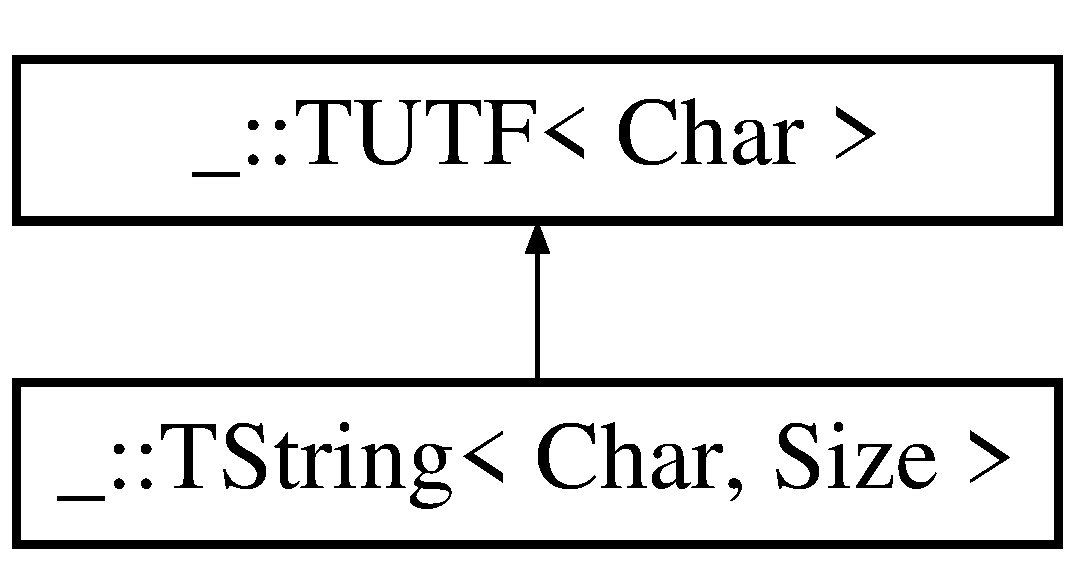
\includegraphics[height=2.000000cm]{class___1_1_t_string}
\end{center}
\end{figure}
\subsection*{Public Member Functions}
\begin{DoxyCompactItemize}
\item 
\mbox{\Hypertarget{class___1_1_t_string_a90e5210f5b757c9abb76637c008bbe57}\label{class___1_1_t_string_a90e5210f5b757c9abb76637c008bbe57}} 
{\bfseries T\+String} (Ascii\+Factory destructor)
\item 
\mbox{\Hypertarget{class___1_1_t_string_aefb5668d73bb76f7c08e9972159862c7}\label{class___1_1_t_string_aefb5668d73bb76f7c08e9972159862c7}} 
{\bfseries T\+String} (S\+IW size, Ascii\+Factory destructor=nullptr)
\item 
\mbox{\Hypertarget{class___1_1_t_string_af42c01ab567cbef7fe4bec027ccf5959}\label{class___1_1_t_string_af42c01ab567cbef7fe4bec027ccf5959}} 
{\bfseries T\+String} (S\+IW size, U\+IW $\ast$buffer, Ascii\+Factory destructor=nullptr)
\item 
\mbox{\Hypertarget{class___1_1_t_string_a81ac61ab0d314c0078d65b64e3daed4a}\label{class___1_1_t_string_a81ac61ab0d314c0078d65b64e3daed4a}} 
\mbox{\hyperlink{struct___1_1_t_u_t_f}{T\+U\+TF}}$<$ Char $>$ {\bfseries Print} ()
\item 
\mbox{\Hypertarget{class___1_1_t_string_a9effab6ba91e83d501aca21674e253c4}\label{class___1_1_t_string_a9effab6ba91e83d501aca21674e253c4}} 
{\footnotesize template$<$typename T $>$ }\\\mbox{\hyperlink{struct___1_1_t_u_t_f}{T\+U\+TF}}$<$ Char $>$ {\bfseries Print} (T item)
\item 
\mbox{\Hypertarget{class___1_1_t_string_aab6602ded5c4c5e7da2e5df06b2d81d5}\label{class___1_1_t_string_aab6602ded5c4c5e7da2e5df06b2d81d5}} 
\mbox{\hyperlink{struct___1_1_t_u_t_f}{T\+U\+TF}}$<$ Char $>$ {\bfseries Print} (Char c)
\item 
\mbox{\Hypertarget{class___1_1_t_string_a2afc6f6903d6d9a8603b74a4033512c2}\label{class___1_1_t_string_a2afc6f6903d6d9a8603b74a4033512c2}} 
\mbox{\hyperlink{struct___1_1_t_u_t_f}{T\+U\+TF}}$<$ Char $>$ {\bfseries Print} (const Char $\ast$string)
\item 
\mbox{\Hypertarget{class___1_1_t_string_a5e635e05910d5142d106708594792178}\label{class___1_1_t_string_a5e635e05910d5142d106708594792178}} 
\mbox{\hyperlink{struct___1_1_t_u_t_f}{T\+U\+TF}}$<$ Char $>$ {\bfseries Print} (S\+I4 value)
\item 
\mbox{\Hypertarget{class___1_1_t_string_a66754382b9205775829f2ae00a39115d}\label{class___1_1_t_string_a66754382b9205775829f2ae00a39115d}} 
\mbox{\hyperlink{struct___1_1_t_u_t_f}{T\+U\+TF}}$<$ Char $>$ {\bfseries Print} (U\+I4 value)
\item 
\mbox{\Hypertarget{class___1_1_t_string_aafc07eecd77440f9fbc1a76a7028ce49}\label{class___1_1_t_string_aafc07eecd77440f9fbc1a76a7028ce49}} 
\mbox{\hyperlink{struct___1_1_t_u_t_f}{T\+U\+TF}}$<$ Char $>$ {\bfseries Print} (S\+I8 value)
\item 
\mbox{\Hypertarget{class___1_1_t_string_a75eda5a9eeac3d39fe6ed869935b5a09}\label{class___1_1_t_string_a75eda5a9eeac3d39fe6ed869935b5a09}} 
\mbox{\hyperlink{struct___1_1_t_u_t_f}{T\+U\+TF}}$<$ Char $>$ {\bfseries Print} (U\+I8 value)
\item 
\mbox{\Hypertarget{class___1_1_t_string_a99f91282240a4bd6e84bbaec5d02ded7}\label{class___1_1_t_string_a99f91282240a4bd6e84bbaec5d02ded7}} 
\mbox{\hyperlink{struct___1_1_t_u_t_f}{T\+U\+TF}}$<$ Char $>$ {\bfseries Print} (F\+LT value)
\item 
\mbox{\Hypertarget{class___1_1_t_string_afec554f47c9360f1ee0fae7e68dcd935}\label{class___1_1_t_string_afec554f47c9360f1ee0fae7e68dcd935}} 
\mbox{\hyperlink{struct___1_1_t_u_t_f}{T\+U\+TF}}$<$ Char $>$ {\bfseries Print} (D\+BL value)
\item 
\mbox{\Hypertarget{class___1_1_t_string_adc42054abf47fc70970d36cb961a666f}\label{class___1_1_t_string_adc42054abf47fc70970d36cb961a666f}} 
Char $\ast$ {\bfseries Stop} ()
\item 
\mbox{\Hypertarget{class___1_1_t_string_af7c39101f3d7de432cc0b8fc0fa251e9}\label{class___1_1_t_string_af7c39101f3d7de432cc0b8fc0fa251e9}} 
Char $\ast$ {\bfseries End} ()
\item 
\mbox{\Hypertarget{class___1_1_t_string_a5170ce88b863a2ca5d8d186542d031df}\label{class___1_1_t_string_a5170ce88b863a2ca5d8d186542d031df}} 
void {\bfseries Terminate} ()
\item 
\mbox{\Hypertarget{class___1_1_t_string_ac201aaf06055455e4cb6ec42a5cad4b4}\label{class___1_1_t_string_ac201aaf06055455e4cb6ec42a5cad4b4}} 
\mbox{\hyperlink{class___1_1_t_object}{T\+Object}}$<$ Size $>$ \& {\bfseries O\+BJ} ()
\end{DoxyCompactItemize}
\subsection*{Additional Inherited Members}


The documentation for this class was generated from the following file\+:\begin{DoxyCompactItemize}
\item 
tutf.\+h\end{DoxyCompactItemize}

\hypertarget{class___1_1_t_token}{}\section{\+\_\+\+:\+:T\+Token$<$ Char $>$ Class Template Reference}
\label{class___1_1_t_token}\index{\+\_\+\+::\+T\+Token$<$ Char $>$@{\+\_\+\+::\+T\+Token$<$ Char $>$}}
\subsection*{Public Member Functions}
\begin{DoxyCompactItemize}
\item 
\mbox{\Hypertarget{class___1_1_t_token_ab36c43426d58dbcf99b06cbcecb9e865}\label{class___1_1_t_token_ab36c43426d58dbcf99b06cbcecb9e865}} 
{\bfseries T\+Token} (Char character)
\item 
\mbox{\Hypertarget{class___1_1_t_token_a892291327a14acf940647ccc4f9c3deb}\label{class___1_1_t_token_a892291327a14acf940647ccc4f9c3deb}} 
{\bfseries T\+Token} (const Char $\ast$string)
\item 
\mbox{\Hypertarget{class___1_1_t_token_ac04afba13e59924ba3b495f7e55d745b}\label{class___1_1_t_token_ac04afba13e59924ba3b495f7e55d745b}} 
{\bfseries T\+Token} (S\+I4 value)
\item 
\mbox{\Hypertarget{class___1_1_t_token_ab53f9e14329030b25fb33b5f84ac86a5}\label{class___1_1_t_token_ab53f9e14329030b25fb33b5f84ac86a5}} 
{\bfseries T\+Token} (U\+I4 value)
\item 
\mbox{\Hypertarget{class___1_1_t_token_a8e69167a25987ded5f50449edf4a14a1}\label{class___1_1_t_token_a8e69167a25987ded5f50449edf4a14a1}} 
{\bfseries T\+Token} (S\+I8 value)
\item 
\mbox{\Hypertarget{class___1_1_t_token_ab112e64da38e901b6485722f0cb9b110}\label{class___1_1_t_token_ab112e64da38e901b6485722f0cb9b110}} 
{\bfseries T\+Token} (U\+I8 value)
\item 
\mbox{\Hypertarget{class___1_1_t_token_a6232132f448c83ad88ce06596f706700}\label{class___1_1_t_token_a6232132f448c83ad88ce06596f706700}} 
{\bfseries T\+Token} (F\+LT value)
\item 
\mbox{\Hypertarget{class___1_1_t_token_aa28d470cb43aa224798cf5d1d66fdaf6}\label{class___1_1_t_token_aa28d470cb43aa224798cf5d1d66fdaf6}} 
{\bfseries T\+Token} (D\+BL value)
\item 
\mbox{\Hypertarget{class___1_1_t_token_ae396613d61c83b9643a880bb91c649ab}\label{class___1_1_t_token_ae396613d61c83b9643a880bb91c649ab}} 
const Char $\ast$ {\bfseries String} ()
\end{DoxyCompactItemize}


The documentation for this class was generated from the following file\+:\begin{DoxyCompactItemize}
\item 
tutf.\+h\end{DoxyCompactItemize}

\hypertarget{struct___1_1_tuple2}{}\section{\+\_\+\+:\+:Tuple2 Struct Reference}
\label{struct___1_1_tuple2}\index{\+\_\+\+::\+Tuple2@{\+\_\+\+::\+Tuple2}}
\subsection*{Public Attributes}
\begin{DoxyCompactItemize}
\item 
\mbox{\Hypertarget{struct___1_1_tuple2_a7707d0df48932fa6f6170c450561a871}\label{struct___1_1_tuple2_a7707d0df48932fa6f6170c450561a871}} 
Ascii\+Type {\bfseries type}
\item 
\mbox{\Hypertarget{struct___1_1_tuple2_a80d9ce7ee73d43fc5b6b6392f3ec54ca}\label{struct___1_1_tuple2_a80d9ce7ee73d43fc5b6b6392f3ec54ca}} 
void $\ast$ {\bfseries value}
\end{DoxyCompactItemize}


The documentation for this struct was generated from the following file\+:\begin{DoxyCompactItemize}
\item 
tset.\+h\end{DoxyCompactItemize}

\hypertarget{struct___1_1_tuple3}{}\section{\+\_\+\+:\+:Tuple3 Struct Reference}
\label{struct___1_1_tuple3}\index{\+\_\+\+::\+Tuple3@{\+\_\+\+::\+Tuple3}}
\subsection*{Public Attributes}
\begin{DoxyCompactItemize}
\item 
\mbox{\Hypertarget{struct___1_1_tuple3_aaab11ab3c99ea6c0128b27f96ffc4142}\label{struct___1_1_tuple3_aaab11ab3c99ea6c0128b27f96ffc4142}} 
Ascii\+Type {\bfseries type}
\item 
\mbox{\Hypertarget{struct___1_1_tuple3_af55cbbd9bfbdde34c3768d5f319a3194}\label{struct___1_1_tuple3_af55cbbd9bfbdde34c3768d5f319a3194}} 
void $\ast$ {\bfseries value}
\item 
\mbox{\Hypertarget{struct___1_1_tuple3_aef8e292e2f9cd542d1f5c7c1cad889ff}\label{struct___1_1_tuple3_aef8e292e2f9cd542d1f5c7c1cad889ff}} 
const char $\ast$ {\bfseries key}
\end{DoxyCompactItemize}


The documentation for this struct was generated from the following file\+:\begin{DoxyCompactItemize}
\item 
tset.\+h\end{DoxyCompactItemize}

\hypertarget{struct___1_1_t_u_t_f}{}\section{\+\_\+\+:\+:T\+U\+TF$<$ Char $>$ Struct Template Reference}
\label{struct___1_1_t_u_t_f}\index{\+\_\+\+::\+T\+U\+T\+F$<$ Char $>$@{\+\_\+\+::\+T\+U\+T\+F$<$ Char $>$}}
Inheritance diagram for \+\_\+\+:\+:T\+U\+TF$<$ Char $>$\+:\begin{figure}[H]
\begin{center}
\leavevmode
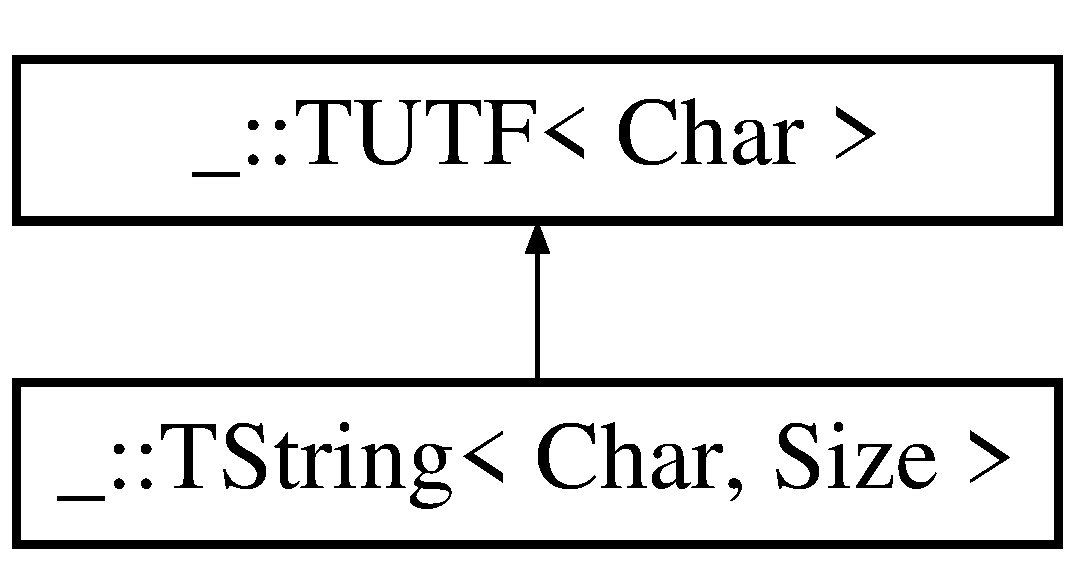
\includegraphics[height=2.000000cm]{struct___1_1_t_u_t_f}
\end{center}
\end{figure}
\subsection*{Public Member Functions}
\begin{DoxyCompactItemize}
\item 
\mbox{\Hypertarget{struct___1_1_t_u_t_f_a39689f4bdee1c84784381d54b44a130f}\label{struct___1_1_t_u_t_f_a39689f4bdee1c84784381d54b44a130f}} 
{\bfseries T\+U\+TF} (Ascii\+Factory memory=T\+S\+Out\+Auto$<$ Char $>$, U\+I8 size=0)
\item 
\mbox{\Hypertarget{struct___1_1_t_u_t_f_a33fdb134f2888f5c99bae2d250ff375b}\label{struct___1_1_t_u_t_f_a33fdb134f2888f5c99bae2d250ff375b}} 
{\bfseries T\+U\+TF} (Char $\ast$begin, S\+IW size)
\item 
\mbox{\Hypertarget{struct___1_1_t_u_t_f_a8676a2619c1aed38d8a55f3d36611128}\label{struct___1_1_t_u_t_f_a8676a2619c1aed38d8a55f3d36611128}} 
{\bfseries T\+U\+TF} (Char $\ast$begin, Char $\ast$end)
\item 
\mbox{\Hypertarget{struct___1_1_t_u_t_f_af3f3eab5a02ce1925a758a7c743b2b74}\label{struct___1_1_t_u_t_f_af3f3eab5a02ce1925a758a7c743b2b74}} 
{\bfseries T\+U\+TF} (const \mbox{\hyperlink{struct___1_1_t_u_t_f}{T\+U\+TF}} \&other)
\item 
\mbox{\Hypertarget{struct___1_1_t_u_t_f_a7aac4c9fea090670ba23b77e48de5ff2}\label{struct___1_1_t_u_t_f_a7aac4c9fea090670ba23b77e48de5ff2}} 
\mbox{\hyperlink{struct___1_1_t_u_t_f}{T\+U\+TF}} \& {\bfseries Set} (Char $\ast$new\+\_\+pointer)
\item 
\mbox{\Hypertarget{struct___1_1_t_u_t_f_ade4df63d5c12600296c8d7d0c861e71d}\label{struct___1_1_t_u_t_f_ade4df63d5c12600296c8d7d0c861e71d}} 
\mbox{\hyperlink{struct___1_1_t_u_t_f}{T\+U\+TF}} \& {\bfseries Hex} (S\+I1 value)
\item 
\mbox{\Hypertarget{struct___1_1_t_u_t_f_afc5c949c3411d293b6b3a1fcd9e75593}\label{struct___1_1_t_u_t_f_afc5c949c3411d293b6b3a1fcd9e75593}} 
\mbox{\hyperlink{struct___1_1_t_u_t_f}{T\+U\+TF}} \& {\bfseries Hex} (U\+I1 value)
\item 
\mbox{\Hypertarget{struct___1_1_t_u_t_f_a585c670a0d8973377a54245b6e30b7ee}\label{struct___1_1_t_u_t_f_a585c670a0d8973377a54245b6e30b7ee}} 
\mbox{\hyperlink{struct___1_1_t_u_t_f}{T\+U\+TF}} \& {\bfseries Hex} (S\+I2 value)
\item 
\mbox{\Hypertarget{struct___1_1_t_u_t_f_a68ba5d60330097402a70f4d9e2d7fdce}\label{struct___1_1_t_u_t_f_a68ba5d60330097402a70f4d9e2d7fdce}} 
\mbox{\hyperlink{struct___1_1_t_u_t_f}{T\+U\+TF}} \& {\bfseries Hex} (U\+I2 value)
\item 
\mbox{\Hypertarget{struct___1_1_t_u_t_f_a92dbf16052496e20228ad9f5c94b988f}\label{struct___1_1_t_u_t_f_a92dbf16052496e20228ad9f5c94b988f}} 
\mbox{\hyperlink{struct___1_1_t_u_t_f}{T\+U\+TF}} \& {\bfseries Hex} (S\+I4 value)
\item 
\mbox{\Hypertarget{struct___1_1_t_u_t_f_ae62b81a17f805b8fe1da6de8a9f4f735}\label{struct___1_1_t_u_t_f_ae62b81a17f805b8fe1da6de8a9f4f735}} 
\mbox{\hyperlink{struct___1_1_t_u_t_f}{T\+U\+TF}} \& {\bfseries Hex} (U\+I4 value)
\item 
\mbox{\Hypertarget{struct___1_1_t_u_t_f_a360528880f85ed48654e367eedc0b264}\label{struct___1_1_t_u_t_f_a360528880f85ed48654e367eedc0b264}} 
\mbox{\hyperlink{struct___1_1_t_u_t_f}{T\+U\+TF}} \& {\bfseries Hex} (S\+I8 value)
\item 
\mbox{\Hypertarget{struct___1_1_t_u_t_f_adf229aa506696d6634cc8423779b5767}\label{struct___1_1_t_u_t_f_adf229aa506696d6634cc8423779b5767}} 
\mbox{\hyperlink{struct___1_1_t_u_t_f}{T\+U\+TF}} \& {\bfseries Hex} (U\+I8 value)
\item 
\mbox{\Hypertarget{struct___1_1_t_u_t_f_a8e49bbec7d5b2c09852e7eea7dd5c843}\label{struct___1_1_t_u_t_f_a8e49bbec7d5b2c09852e7eea7dd5c843}} 
\mbox{\hyperlink{struct___1_1_t_u_t_f}{T\+U\+TF}} \& {\bfseries Hex} (F\+LT value)
\item 
\mbox{\Hypertarget{struct___1_1_t_u_t_f_aebeca6d08a28329879799707c769fef5}\label{struct___1_1_t_u_t_f_aebeca6d08a28329879799707c769fef5}} 
\mbox{\hyperlink{struct___1_1_t_u_t_f}{T\+U\+TF}} \& {\bfseries Hex} (D\+BL value)
\item 
\mbox{\Hypertarget{struct___1_1_t_u_t_f_ac9c96b51950a811deff73dd5943be9a8}\label{struct___1_1_t_u_t_f_ac9c96b51950a811deff73dd5943be9a8}} 
\mbox{\hyperlink{struct___1_1_t_u_t_f}{T\+U\+TF}} \& {\bfseries Hex} (const void $\ast$value)
\item 
\mbox{\Hypertarget{struct___1_1_t_u_t_f_a132cfbc97edc4491cd48b60ba117d2c0}\label{struct___1_1_t_u_t_f_a132cfbc97edc4491cd48b60ba117d2c0}} 
\mbox{\hyperlink{struct___1_1_t_u_t_f}{T\+U\+TF}} \& {\bfseries Binary} (S\+I1 value)
\item 
\mbox{\Hypertarget{struct___1_1_t_u_t_f_a3cdd502c85f52feeb63e08e8a28b3fde}\label{struct___1_1_t_u_t_f_a3cdd502c85f52feeb63e08e8a28b3fde}} 
\mbox{\hyperlink{struct___1_1_t_u_t_f}{T\+U\+TF}} \& {\bfseries Binary} (U\+I1 value)
\item 
\mbox{\Hypertarget{struct___1_1_t_u_t_f_a45971891d86f1aa579e39317c044e973}\label{struct___1_1_t_u_t_f_a45971891d86f1aa579e39317c044e973}} 
\mbox{\hyperlink{struct___1_1_t_u_t_f}{T\+U\+TF}} \& {\bfseries Binary} (S\+I2 value)
\item 
\mbox{\Hypertarget{struct___1_1_t_u_t_f_a0c7d211355105fa9977331f0c8e8d592}\label{struct___1_1_t_u_t_f_a0c7d211355105fa9977331f0c8e8d592}} 
\mbox{\hyperlink{struct___1_1_t_u_t_f}{T\+U\+TF}} \& {\bfseries Binary} (U\+I2 value)
\item 
\mbox{\Hypertarget{struct___1_1_t_u_t_f_a6c8d9d534aa7e775af896a83462954c1}\label{struct___1_1_t_u_t_f_a6c8d9d534aa7e775af896a83462954c1}} 
\mbox{\hyperlink{struct___1_1_t_u_t_f}{T\+U\+TF}} \& {\bfseries Binary} (S\+I4 value)
\item 
\mbox{\Hypertarget{struct___1_1_t_u_t_f_abf686fe4bb21e8edb06a7521ec082f72}\label{struct___1_1_t_u_t_f_abf686fe4bb21e8edb06a7521ec082f72}} 
\mbox{\hyperlink{struct___1_1_t_u_t_f}{T\+U\+TF}} \& {\bfseries Binary} (U\+I4 value)
\item 
\mbox{\Hypertarget{struct___1_1_t_u_t_f_ad7c1b1c4898e07fd50b14460eb7d38b5}\label{struct___1_1_t_u_t_f_ad7c1b1c4898e07fd50b14460eb7d38b5}} 
\mbox{\hyperlink{struct___1_1_t_u_t_f}{T\+U\+TF}} \& {\bfseries Binary} (S\+I8 value)
\item 
\mbox{\Hypertarget{struct___1_1_t_u_t_f_a8488be27f536e84b2842e2f0afae7b49}\label{struct___1_1_t_u_t_f_a8488be27f536e84b2842e2f0afae7b49}} 
\mbox{\hyperlink{struct___1_1_t_u_t_f}{T\+U\+TF}} \& {\bfseries Binary} (U\+I8 value)
\item 
\mbox{\Hypertarget{struct___1_1_t_u_t_f_a8edfbe73971ce6db7c2f6aafd3c5941f}\label{struct___1_1_t_u_t_f_a8edfbe73971ce6db7c2f6aafd3c5941f}} 
\mbox{\hyperlink{struct___1_1_t_u_t_f}{T\+U\+TF}} \& {\bfseries Binary} (F\+LT value)
\item 
\mbox{\Hypertarget{struct___1_1_t_u_t_f_a049f47814d4721d454de5732c8469451}\label{struct___1_1_t_u_t_f_a049f47814d4721d454de5732c8469451}} 
\mbox{\hyperlink{struct___1_1_t_u_t_f}{T\+U\+TF}} \& {\bfseries Binary} (D\+BL value)
\item 
\mbox{\Hypertarget{struct___1_1_t_u_t_f_a1d24b1ef65ca5411f7cff2664ff123af}\label{struct___1_1_t_u_t_f_a1d24b1ef65ca5411f7cff2664ff123af}} 
\mbox{\hyperlink{struct___1_1_t_u_t_f}{T\+U\+TF}} \& {\bfseries Binary} (const void $\ast$value)
\end{DoxyCompactItemize}
\subsection*{Public Attributes}
\begin{DoxyCompactItemize}
\item 
\mbox{\Hypertarget{struct___1_1_t_u_t_f_a75e6d2718260a484653e7f904ed08948}\label{struct___1_1_t_u_t_f_a75e6d2718260a484653e7f904ed08948}} 
Char $\ast$ {\bfseries begin}
\item 
\mbox{\Hypertarget{struct___1_1_t_u_t_f_a585e320e42fb4e57d7170bcd7bc4852f}\label{struct___1_1_t_u_t_f_a585e320e42fb4e57d7170bcd7bc4852f}} 
Char $\ast$ {\bfseries end}
\end{DoxyCompactItemize}


The documentation for this struct was generated from the following file\+:\begin{DoxyCompactItemize}
\item 
tutf.\+h\end{DoxyCompactItemize}

\hypertarget{struct___1_1_u_t_f1}{}\section{\+\_\+\+:\+:U\+T\+F1 Struct Reference}
\label{struct___1_1_u_t_f1}\index{\+\_\+\+::\+U\+T\+F1@{\+\_\+\+::\+U\+T\+F1}}
\subsection*{Public Member Functions}
\begin{DoxyCompactItemize}
\item 
\mbox{\Hypertarget{struct___1_1_u_t_f1_a6877af0a99a95ba66ff31a0ea3792233}\label{struct___1_1_u_t_f1_a6877af0a99a95ba66ff31a0ea3792233}} 
{\bfseries U\+T\+F1} (char $\ast$begin, size\+\_\+t size)
\item 
\mbox{\Hypertarget{struct___1_1_u_t_f1_ae51619e58bc986876998474bf2978331}\label{struct___1_1_u_t_f1_ae51619e58bc986876998474bf2978331}} 
{\bfseries U\+T\+F1} (char $\ast$begin, char $\ast$end)
\item 
\mbox{\Hypertarget{struct___1_1_u_t_f1_a047c4a4adebe9682ae51d518fafab86c}\label{struct___1_1_u_t_f1_a047c4a4adebe9682ae51d518fafab86c}} 
{\bfseries U\+T\+F1} (const \mbox{\hyperlink{struct___1_1_u_t_f1}{U\+T\+F1}} \&other)
\item 
\mbox{\Hypertarget{struct___1_1_u_t_f1_ae85362362dd9dd2128da2feb9df575ee}\label{struct___1_1_u_t_f1_ae85362362dd9dd2128da2feb9df575ee}} 
\mbox{\hyperlink{struct___1_1_u_t_f1}{U\+T\+F1}} \& {\bfseries Set} (char $\ast$new\+\_\+pointer)
\item 
\mbox{\Hypertarget{struct___1_1_u_t_f1_a02a651e0e0a1c0ba03b09050505ae746}\label{struct___1_1_u_t_f1_a02a651e0e0a1c0ba03b09050505ae746}} 
\mbox{\hyperlink{struct___1_1_u_t_f1}{U\+T\+F1}} \& {\bfseries Hex} (S\+I1 value)
\item 
\mbox{\Hypertarget{struct___1_1_u_t_f1_ad49bed1a684fc41f15f7de7698147e09}\label{struct___1_1_u_t_f1_ad49bed1a684fc41f15f7de7698147e09}} 
\mbox{\hyperlink{struct___1_1_u_t_f1}{U\+T\+F1}} \& {\bfseries Hex} (U\+I1 value)
\item 
\mbox{\Hypertarget{struct___1_1_u_t_f1_aa9bf83cc9c6c70aa807cf32708ecefbe}\label{struct___1_1_u_t_f1_aa9bf83cc9c6c70aa807cf32708ecefbe}} 
\mbox{\hyperlink{struct___1_1_u_t_f1}{U\+T\+F1}} \& {\bfseries Hex} (S\+I2 value)
\item 
\mbox{\Hypertarget{struct___1_1_u_t_f1_a98cee4f7cf838f940858206cacc44240}\label{struct___1_1_u_t_f1_a98cee4f7cf838f940858206cacc44240}} 
\mbox{\hyperlink{struct___1_1_u_t_f1}{U\+T\+F1}} \& {\bfseries Hex} (U\+I2 value)
\item 
\mbox{\Hypertarget{struct___1_1_u_t_f1_a34ffa4125bee4ab7e8edc184ba9d4c9d}\label{struct___1_1_u_t_f1_a34ffa4125bee4ab7e8edc184ba9d4c9d}} 
\mbox{\hyperlink{struct___1_1_u_t_f1}{U\+T\+F1}} \& {\bfseries Hex} (S\+I4 value)
\item 
\mbox{\Hypertarget{struct___1_1_u_t_f1_a7a2d490991ae269c46d769c4b7cabf6a}\label{struct___1_1_u_t_f1_a7a2d490991ae269c46d769c4b7cabf6a}} 
\mbox{\hyperlink{struct___1_1_u_t_f1}{U\+T\+F1}} \& {\bfseries Hex} (U\+I4 value)
\item 
\mbox{\Hypertarget{struct___1_1_u_t_f1_abb67d72fb739a43c16f0dd9381139b92}\label{struct___1_1_u_t_f1_abb67d72fb739a43c16f0dd9381139b92}} 
\mbox{\hyperlink{struct___1_1_u_t_f1}{U\+T\+F1}} \& {\bfseries Hex} (S\+I8 value)
\item 
\mbox{\Hypertarget{struct___1_1_u_t_f1_ab2c31f3727b13293b05a3b3806c36038}\label{struct___1_1_u_t_f1_ab2c31f3727b13293b05a3b3806c36038}} 
\mbox{\hyperlink{struct___1_1_u_t_f1}{U\+T\+F1}} \& {\bfseries Hex} (U\+I8 value)
\item 
\mbox{\Hypertarget{struct___1_1_u_t_f1_a4bc261c6c980aa3d20f00f4d3c457d64}\label{struct___1_1_u_t_f1_a4bc261c6c980aa3d20f00f4d3c457d64}} 
\mbox{\hyperlink{struct___1_1_u_t_f1}{U\+T\+F1}} \& {\bfseries Hex} (F\+LT value)
\item 
\mbox{\Hypertarget{struct___1_1_u_t_f1_ae669a669851e036cface4e7ade953f12}\label{struct___1_1_u_t_f1_ae669a669851e036cface4e7ade953f12}} 
\mbox{\hyperlink{struct___1_1_u_t_f1}{U\+T\+F1}} \& {\bfseries Hex} (D\+BL value)
\item 
\mbox{\Hypertarget{struct___1_1_u_t_f1_a5eb01ac5dff8a7a0ff3f6f084dd42583}\label{struct___1_1_u_t_f1_a5eb01ac5dff8a7a0ff3f6f084dd42583}} 
\mbox{\hyperlink{struct___1_1_u_t_f1}{U\+T\+F1}} \& {\bfseries Hex} (const void $\ast$pointer)
\item 
\mbox{\Hypertarget{struct___1_1_u_t_f1_afb6331bdbf98e4ab0636a058dffb49f3}\label{struct___1_1_u_t_f1_afb6331bdbf98e4ab0636a058dffb49f3}} 
\mbox{\hyperlink{struct___1_1_u_t_f1}{U\+T\+F1}} \& {\bfseries Binary} (S\+I1 value)
\item 
\mbox{\Hypertarget{struct___1_1_u_t_f1_a8e0fa898eed8a8cd652f0ce49ff81077}\label{struct___1_1_u_t_f1_a8e0fa898eed8a8cd652f0ce49ff81077}} 
\mbox{\hyperlink{struct___1_1_u_t_f1}{U\+T\+F1}} \& {\bfseries Binary} (U\+I1 value)
\item 
\mbox{\Hypertarget{struct___1_1_u_t_f1_a033a530a803118432128eb299d5856b7}\label{struct___1_1_u_t_f1_a033a530a803118432128eb299d5856b7}} 
\mbox{\hyperlink{struct___1_1_u_t_f1}{U\+T\+F1}} \& {\bfseries Binary} (S\+I2 value)
\item 
\mbox{\Hypertarget{struct___1_1_u_t_f1_ab8dab2b3b096a5a195b88ec5cde40d57}\label{struct___1_1_u_t_f1_ab8dab2b3b096a5a195b88ec5cde40d57}} 
\mbox{\hyperlink{struct___1_1_u_t_f1}{U\+T\+F1}} \& {\bfseries Binary} (U\+I2 value)
\item 
\mbox{\Hypertarget{struct___1_1_u_t_f1_afb5c8bd995f7cfe9978302204848dd1c}\label{struct___1_1_u_t_f1_afb5c8bd995f7cfe9978302204848dd1c}} 
\mbox{\hyperlink{struct___1_1_u_t_f1}{U\+T\+F1}} \& {\bfseries Binary} (S\+I4 value)
\item 
\mbox{\Hypertarget{struct___1_1_u_t_f1_a2c33327c9edbab8368e03fb96d6aa43a}\label{struct___1_1_u_t_f1_a2c33327c9edbab8368e03fb96d6aa43a}} 
\mbox{\hyperlink{struct___1_1_u_t_f1}{U\+T\+F1}} \& {\bfseries Binary} (U\+I4 value)
\item 
\mbox{\Hypertarget{struct___1_1_u_t_f1_a5dbf6df17c26073995aab00f13dac37a}\label{struct___1_1_u_t_f1_a5dbf6df17c26073995aab00f13dac37a}} 
\mbox{\hyperlink{struct___1_1_u_t_f1}{U\+T\+F1}} \& {\bfseries Binary} (S\+I8 value)
\item 
\mbox{\Hypertarget{struct___1_1_u_t_f1_a4c5d98d70695a89f6967a54c4c33bb23}\label{struct___1_1_u_t_f1_a4c5d98d70695a89f6967a54c4c33bb23}} 
\mbox{\hyperlink{struct___1_1_u_t_f1}{U\+T\+F1}} \& {\bfseries Binary} (U\+I8 value)
\item 
\mbox{\Hypertarget{struct___1_1_u_t_f1_a3a68b3b28f1bae0f61f95529d5bc2b45}\label{struct___1_1_u_t_f1_a3a68b3b28f1bae0f61f95529d5bc2b45}} 
\mbox{\hyperlink{struct___1_1_u_t_f1}{U\+T\+F1}} \& {\bfseries Binary} (F\+LT value)
\item 
\mbox{\Hypertarget{struct___1_1_u_t_f1_a94f60b89bc73947589700b4cf23994e1}\label{struct___1_1_u_t_f1_a94f60b89bc73947589700b4cf23994e1}} 
\mbox{\hyperlink{struct___1_1_u_t_f1}{U\+T\+F1}} \& {\bfseries Binary} (D\+BL value)
\item 
\mbox{\Hypertarget{struct___1_1_u_t_f1_a987b52f2e3707b8b2bd6befd03fd567c}\label{struct___1_1_u_t_f1_a987b52f2e3707b8b2bd6befd03fd567c}} 
\mbox{\hyperlink{struct___1_1_u_t_f1}{U\+T\+F1}} \& {\bfseries Binary} (const void $\ast$pointer)
\end{DoxyCompactItemize}
\subsection*{Public Attributes}
\begin{DoxyCompactItemize}
\item 
\mbox{\Hypertarget{struct___1_1_u_t_f1_a74b5cb45155d78d9893712dd42204f16}\label{struct___1_1_u_t_f1_a74b5cb45155d78d9893712dd42204f16}} 
char $\ast$ {\bfseries begin}
\item 
\mbox{\Hypertarget{struct___1_1_u_t_f1_a837b875819850938844feb52a6629c85}\label{struct___1_1_u_t_f1_a837b875819850938844feb52a6629c85}} 
char $\ast$ {\bfseries end}
\end{DoxyCompactItemize}


The documentation for this struct was generated from the following files\+:\begin{DoxyCompactItemize}
\item 
cutf1.\+h\item 
script2\+\_\+utf.\+cc\end{DoxyCompactItemize}

\hypertarget{class___1_1_utf8_center}{}\section{\+\_\+\+:\+:Utf8\+Center Class Reference}
\label{class___1_1_utf8_center}\index{\+\_\+\+::\+Utf8\+Center@{\+\_\+\+::\+Utf8\+Center}}
\subsection*{Public Member Functions}
\begin{DoxyCompactItemize}
\item 
\mbox{\Hypertarget{class___1_1_utf8_center_ad5e858bf3824593671c566c5d14a43a5}\label{class___1_1_utf8_center_ad5e858bf3824593671c566c5d14a43a5}} 
{\bfseries Utf8\+Center} (const char $\ast$string, int column\+\_\+count)
\item 
\mbox{\Hypertarget{class___1_1_utf8_center_a9b92822c7e89e698c7290df5ba51c013}\label{class___1_1_utf8_center_a9b92822c7e89e698c7290df5ba51c013}} 
{\bfseries Utf8\+Center} (S\+I4 value, int column\+\_\+count)
\item 
\mbox{\Hypertarget{class___1_1_utf8_center_ae40b2338ee2e32a00a9a4e514fbb6236}\label{class___1_1_utf8_center_ae40b2338ee2e32a00a9a4e514fbb6236}} 
{\bfseries Utf8\+Center} (U\+I4 value, int column\+\_\+count)
\item 
\mbox{\Hypertarget{class___1_1_utf8_center_af607fa10a6d81b526be6ab778929d7fb}\label{class___1_1_utf8_center_af607fa10a6d81b526be6ab778929d7fb}} 
{\bfseries Utf8\+Center} (S\+I8 value, int column\+\_\+count)
\item 
\mbox{\Hypertarget{class___1_1_utf8_center_aa1e81b57e33c0ce5c07be9117a7bb39c}\label{class___1_1_utf8_center_aa1e81b57e33c0ce5c07be9117a7bb39c}} 
{\bfseries Utf8\+Center} (U\+I8 value, int column\+\_\+count)
\item 
\mbox{\Hypertarget{class___1_1_utf8_center_a2fdb089f1029fb8a6aa504a75e4c50d0}\label{class___1_1_utf8_center_a2fdb089f1029fb8a6aa504a75e4c50d0}} 
{\bfseries Utf8\+Center} (F\+LT value, int column\+\_\+count)
\item 
\mbox{\Hypertarget{class___1_1_utf8_center_a7b1068a4c47be97866e800bce65b9dcb}\label{class___1_1_utf8_center_a7b1068a4c47be97866e800bce65b9dcb}} 
{\bfseries Utf8\+Center} (D\+BL value, int column\+\_\+count)
\item 
\mbox{\Hypertarget{class___1_1_utf8_center_a6dd6751c749bfcd6993ddf7bfffe05fa}\label{class___1_1_utf8_center_a6dd6751c749bfcd6993ddf7bfffe05fa}} 
const char $\ast$ {\bfseries String} ()
\item 
\mbox{\Hypertarget{class___1_1_utf8_center_a2a40b1dbbada10b48944aa4d5e47f42f}\label{class___1_1_utf8_center_a2a40b1dbbada10b48944aa4d5e47f42f}} 
int {\bfseries Get\+Column\+Count} ()
\end{DoxyCompactItemize}


The documentation for this class was generated from the following files\+:\begin{DoxyCompactItemize}
\item 
cutf1.\+h\item 
script2\+\_\+utf.\+cc\end{DoxyCompactItemize}

\hypertarget{struct___1_1_utf8_line}{}\section{\+\_\+\+:\+:Utf8\+Line Struct Reference}
\label{struct___1_1_utf8_line}\index{\+\_\+\+::\+Utf8\+Line@{\+\_\+\+::\+Utf8\+Line}}
\subsection*{Public Member Functions}
\begin{DoxyCompactItemize}
\item 
\mbox{\Hypertarget{struct___1_1_utf8_line_a34c6478ca0f09c7d36654ed47f6f7fdf}\label{struct___1_1_utf8_line_a34c6478ca0f09c7d36654ed47f6f7fdf}} 
{\bfseries Utf8\+Line} (char token, int column\+\_\+count)
\end{DoxyCompactItemize}
\subsection*{Public Attributes}
\begin{DoxyCompactItemize}
\item 
\mbox{\Hypertarget{struct___1_1_utf8_line_a4c2bc24fda62b1031f1a121ae1da61fc}\label{struct___1_1_utf8_line_a4c2bc24fda62b1031f1a121ae1da61fc}} 
char {\bfseries token}
\item 
\mbox{\Hypertarget{struct___1_1_utf8_line_ada87b911edf08166ff5a01dfba8b7836}\label{struct___1_1_utf8_line_ada87b911edf08166ff5a01dfba8b7836}} 
int {\bfseries column\+\_\+count}
\end{DoxyCompactItemize}


The documentation for this struct was generated from the following files\+:\begin{DoxyCompactItemize}
\item 
cutf1.\+h\item 
script2\+\_\+utf.\+cc\end{DoxyCompactItemize}

\hypertarget{struct___1_1_utf8_line_string}{}\section{\+\_\+\+:\+:Utf8\+Line\+String Struct Reference}
\label{struct___1_1_utf8_line_string}\index{\+\_\+\+::\+Utf8\+Line\+String@{\+\_\+\+::\+Utf8\+Line\+String}}
\subsection*{Public Member Functions}
\begin{DoxyCompactItemize}
\item 
\mbox{\Hypertarget{struct___1_1_utf8_line_string_af4dab13dfcf255845a8ac126282c19c9}\label{struct___1_1_utf8_line_string_af4dab13dfcf255845a8ac126282c19c9}} 
{\bfseries Utf8\+Line\+String} (const char $\ast$string, int column\+\_\+count)
\end{DoxyCompactItemize}
\subsection*{Public Attributes}
\begin{DoxyCompactItemize}
\item 
\mbox{\Hypertarget{struct___1_1_utf8_line_string_a4dcedf89e8915275029abad2d8131a7b}\label{struct___1_1_utf8_line_string_a4dcedf89e8915275029abad2d8131a7b}} 
const char $\ast$ {\bfseries string}
\item 
\mbox{\Hypertarget{struct___1_1_utf8_line_string_a1adeae247199eed43cd3e273c817b343}\label{struct___1_1_utf8_line_string_a1adeae247199eed43cd3e273c817b343}} 
int {\bfseries column\+\_\+count}
\end{DoxyCompactItemize}


The documentation for this struct was generated from the following files\+:\begin{DoxyCompactItemize}
\item 
cutf1.\+h\item 
script2\+\_\+utf.\+cc\end{DoxyCompactItemize}

\hypertarget{class___1_1_utf8_right}{}\section{\+\_\+\+:\+:Utf8\+Right Class Reference}
\label{class___1_1_utf8_right}\index{\+\_\+\+::\+Utf8\+Right@{\+\_\+\+::\+Utf8\+Right}}
\subsection*{Public Member Functions}
\begin{DoxyCompactItemize}
\item 
\mbox{\Hypertarget{class___1_1_utf8_right_a2a760af0a5a9eda2702ddd7f24681f8a}\label{class___1_1_utf8_right_a2a760af0a5a9eda2702ddd7f24681f8a}} 
{\bfseries Utf8\+Right} (const char $\ast$string, int column\+\_\+count)
\item 
\mbox{\Hypertarget{class___1_1_utf8_right_a3effee4485e06c9d644a8a5ced09f935}\label{class___1_1_utf8_right_a3effee4485e06c9d644a8a5ced09f935}} 
{\bfseries Utf8\+Right} (S\+I4 value, int column\+\_\+count)
\item 
\mbox{\Hypertarget{class___1_1_utf8_right_ab5dceadaa31221751de9ffe8a7be535c}\label{class___1_1_utf8_right_ab5dceadaa31221751de9ffe8a7be535c}} 
{\bfseries Utf8\+Right} (U\+I4 value, int column\+\_\+count)
\item 
\mbox{\Hypertarget{class___1_1_utf8_right_a7fa135eb0eca41399a597394330ac861}\label{class___1_1_utf8_right_a7fa135eb0eca41399a597394330ac861}} 
{\bfseries Utf8\+Right} (S\+I8 value, int column\+\_\+count)
\item 
\mbox{\Hypertarget{class___1_1_utf8_right_abe7a5d5bba859b840fd873db260b8a60}\label{class___1_1_utf8_right_abe7a5d5bba859b840fd873db260b8a60}} 
{\bfseries Utf8\+Right} (U\+I8 value, int column\+\_\+count)
\item 
\mbox{\Hypertarget{class___1_1_utf8_right_ab9bc178215a255c901eb3840681fa6a2}\label{class___1_1_utf8_right_ab9bc178215a255c901eb3840681fa6a2}} 
{\bfseries Utf8\+Right} (F\+LT value, int column\+\_\+count)
\item 
\mbox{\Hypertarget{class___1_1_utf8_right_a24e233b3ae3aa23c3a81baa7126686cb}\label{class___1_1_utf8_right_a24e233b3ae3aa23c3a81baa7126686cb}} 
{\bfseries Utf8\+Right} (D\+BL value, int column\+\_\+count)
\item 
\mbox{\Hypertarget{class___1_1_utf8_right_a113f3f1ba3aeba9fbf2a53156b6da82d}\label{class___1_1_utf8_right_a113f3f1ba3aeba9fbf2a53156b6da82d}} 
const char $\ast$ {\bfseries String} ()
\item 
\mbox{\Hypertarget{class___1_1_utf8_right_a782ebf21f4d6c629a11373215d5b9ebd}\label{class___1_1_utf8_right_a782ebf21f4d6c629a11373215d5b9ebd}} 
int {\bfseries Get\+Column\+Count} ()
\end{DoxyCompactItemize}


The documentation for this class was generated from the following files\+:\begin{DoxyCompactItemize}
\item 
cutf1.\+h\item 
script2\+\_\+utf.\+cc\end{DoxyCompactItemize}

\hypertarget{class___1_1_utf8_text}{}\section{\+\_\+\+:\+:Utf8\+Text Class Reference}
\label{class___1_1_utf8_text}\index{\+\_\+\+::\+Utf8\+Text@{\+\_\+\+::\+Utf8\+Text}}
\subsection*{Public Member Functions}
\begin{DoxyCompactItemize}
\item 
\mbox{\Hypertarget{class___1_1_utf8_text_a36ee98ee75033dad969e3c8b19882837}\label{class___1_1_utf8_text_a36ee98ee75033dad969e3c8b19882837}} 
{\bfseries Utf8\+Text} (char character)
\item 
\mbox{\Hypertarget{class___1_1_utf8_text_a92045406e5433109be4ffdac6bca3d7a}\label{class___1_1_utf8_text_a92045406e5433109be4ffdac6bca3d7a}} 
{\bfseries Utf8\+Text} (S\+I4 value)
\item 
\mbox{\Hypertarget{class___1_1_utf8_text_a1cbc14dfeab144956d558e187f9901af}\label{class___1_1_utf8_text_a1cbc14dfeab144956d558e187f9901af}} 
{\bfseries Utf8\+Text} (U\+I4 value)
\item 
\mbox{\Hypertarget{class___1_1_utf8_text_a1146c2ec0ad83a749feda61df3b8441e}\label{class___1_1_utf8_text_a1146c2ec0ad83a749feda61df3b8441e}} 
{\bfseries Utf8\+Text} (S\+I8 value)
\item 
\mbox{\Hypertarget{class___1_1_utf8_text_aa61f92689a406224e6cfadc7d916cd9a}\label{class___1_1_utf8_text_aa61f92689a406224e6cfadc7d916cd9a}} 
{\bfseries Utf8\+Text} (U\+I8 value)
\item 
\mbox{\Hypertarget{class___1_1_utf8_text_a8b760c7132b60e2c27bd3f9cfd503d36}\label{class___1_1_utf8_text_a8b760c7132b60e2c27bd3f9cfd503d36}} 
{\bfseries Utf8\+Text} (F\+LT value)
\item 
\mbox{\Hypertarget{class___1_1_utf8_text_ad1576548492b0e43b16884eacc3dfe3d}\label{class___1_1_utf8_text_ad1576548492b0e43b16884eacc3dfe3d}} 
{\bfseries Utf8\+Text} (D\+BL value)
\item 
\mbox{\Hypertarget{class___1_1_utf8_text_aaef31248826ab19834aa7b78df44b921}\label{class___1_1_utf8_text_aaef31248826ab19834aa7b78df44b921}} 
const char $\ast$ {\bfseries String} ()
\end{DoxyCompactItemize}


The documentation for this class was generated from the following files\+:\begin{DoxyCompactItemize}
\item 
cutf1.\+h\item 
script2\+\_\+utf.\+cc\end{DoxyCompactItemize}

\chapter{File Documentation}
\hypertarget{script2__morsecode_8cc}{}\section{script2\+\_\+morsecode.\+cc File Reference}
\label{script2__morsecode_8cc}\index{script2\+\_\+morsecode.\+cc@{script2\+\_\+morsecode.\+cc}}
{\ttfamily \#include $<$pch.\+h$>$}\newline
\subsection*{Functions}
\begin{DoxyCompactItemize}
\item 
\mbox{\Hypertarget{script2__morsecode_8cc_adb7e92dc52082c8e81ffee1734b52c11}\label{script2__morsecode_8cc_adb7e92dc52082c8e81ffee1734b52c11}} 
const char $\ast$ {\bfseries \+\_\+\+::\+To\+Morse\+Code} (char code)
\end{DoxyCompactItemize}


\subsection{Detailed Description}
Script \begin{DoxyVersion}{Version}
0.\+x \mbox{\hyperlink{}{Cale Mc\+Collough \href{mailto:cale.mccollough@gmail.com}{\tt cale.\+mccollough@gmail.\+com}  Copyright (C) 2014-\/2017 Cale Mc\+Collough $<$calemccollough.\+github.\+io$>$; All right reserved (R). Licensed under the Apache License, Version 2.\+0 (the \char`\"{}\+License\char`\"{}); you may not use this file except in compliance with the License. You may obtain a copy of the License at www.\+apache.\+org/licenses/\+L\+I\+C\+E\+N\+S\+E-\/2.0. Unless required by applicable law or agreed to in writing, software distributed under the License is distributed on an \char`\"{}\+A\+S I\+S\char`\"{} B\+A\+S\+IS, W\+I\+T\+H\+O\+UT W\+A\+R\+R\+A\+N\+T\+I\+ES OR C\+O\+N\+D\+I\+T\+I\+O\+NS OF A\+NY K\+I\+ND, either express or implied. See the License for the specific language governing permissions and limitations under the License. }}
\end{DoxyVersion}

%--- End generated contents ---

% Index
\backmatter
\newpage
\phantomsection
\clearemptydoublepage
\addcontentsline{toc}{chapter}{Index}
\printindex

\end{document}
